\documentclass[    
    paper=a4,
    %landscape,
    %twocolumn,
    twoside=false,
    %BCOR=10mm,
    12pt,
    pagesize=auto,
    parskip=half,
    headsepline=true,
    numbers=noenddot, % enddot, noenddot
    draft=false
]{report}

%-------------------------------------------------------
% Spacing
%-------------------------------------------------------
\setlength{\parindent}{2em}
\setlength{\parskip}{0.5em}

%-------------------------------------------------------
% Graphics
%-------------------------------------------------------
% For \includegraphics{}
\usepackage[pdftex]{graphicx}
\usepackage{subfigure}

% Set Path for Pictures
\graphicspath{{Images/}}

% include PDFs
\usepackage{pdfpages}

%-------------------------------------------------------
% Tables
%-------------------------------------------------------
\usepackage{csvsimple}
%\usepackage[table,xcdraw]{xcolor}

%-------------------------------------------------------
% Maths
%-------------------------------------------------------
\usepackage{amsmath}
\usepackage{siunitx}
\usepackage{physics}

%-------------------------------------------------------
% Code
%-------------------------------------------------------
\usepackage{algorithm}
\usepackage{algorithmic}

%-------------------------------------------------------
% Font
%-------------------------------------------------------
\usepackage[T1]{fontenc}
\usepackage[top=5cm, bottom=4cm, left=3cm, right=3cm]{geometry}

%-------------------------------------------------------
% Spelling
%-------------------------------------------------------
\usepackage[english]{babel}

%-------------------------------------------------------
% Bibliography
%-------------------------------------------------------
\usepackage[noadjust]{cite}
\bibliographystyle{IEEEtran}

%-------------------------------------------------------
% Appendix
%-------------------------------------------------------
\usepackage[toc,page]{appendix}

%-------------------------------------------------------
% Header
%-------------------------------------------------------
\usepackage{fancyhdr}
\pagestyle{fancy}
\fancyhf{}
\lhead{\leftmark}
\rhead{\thepage}
\setlength{\headheight}{15pt}

%-------------------------------------------------------
% Reference
%-------------------------------------------------------
\usepackage[hidelinks]{hyperref}

%-------------------------------------------------------
% Caption
%-------------------------------------------------------
\usepackage{caption}

%-------------------------------------------------------
% Roman Numbers
%------------------------------------------------------
\makeatletter
\newcommand*{\rom}[1]{\expandafter\@slowromancap\romannumeral #1@}
\makeatother

%-------------------------------------------------------
% Parameter
%-------------------------------------------------------
\title{ARIS - Localization of a Sounding Rocket via GPS}
\author{Simon Herzog}
\date{\today}


\begin{document}
 
 % Start with roman page numbering and reset counter
 \setcounter{page}{1}
 \pagenumbering{roman}
 
 %----------------------------------------------------------------------------------------
%	TITLE PAGE
%----------------------------------------------------------------------------------------

\begin{titlepage} % Suppresses displaying the page number on the title page and the subsequent page counts as page 1
	\newcommand{\HRule}{\rule{\linewidth}{0.5mm}} % Defines a new command for horizontal lines, change thickness here
	
	\center % Centre everything on the page
	
	\textsc{\large Lucerne University of\\ Applied Sciences and Arts}\\[0.2cm] % Main heading such as the name of your university/college
	
	%------------------------------------------------
	%	Title
	%------------------------------------------------
	
	\HRule\\[0.4cm]
	
	{\LARGE\bfseries Localization of a Sounding Rocket via GPS}\\[0.4cm] % Title of your document
	
	\HRule\\[0.5cm]
	
	\large \textsc{\textbf{Bachelor Thesis}}\\[0.5cm] 
	
	\vfill
	
	\begin{figure}[!h]
	  \centering
	  
\includegraphics[height=7cm]{images/Tell_Logo.png}
	\end{figure}
	
	\vfill
	
	\textsc{\normalsize Simon Herzog}\\[0.3cm]
	
	{\normalsize Department}\\
	
	\textsc{\normalsize Electrical engineering and information technology}\\[0.3cm] % Major heading such as course name
	
	\vfill
	
	%------------------------------------------------
	%	Supervisors
	%------------------------------------------------
	
	\begin{minipage}{0.4\textwidth}
		\begin{flushleft}
			\normalsize
			\textit{Supervisor}\\
			\textsc{Prof.} M. \textsc{Joss} % Supervisor's name
			\vspace{4mm}\\
			\normalsize
			\textit{Expert}\\
			W. \textsc{Scheidegger} % Expert's name
		\end{flushleft}
	\end{minipage}
	~
	\begin{minipage}{0.4\textwidth}
		\begin{flushright}
			\normalsize
			\textit{Industry Partner}\\
			O. \textsc{Kirchhoff}\\
			CEO ARIS
		\end{flushright}
	\end{minipage}
	
	\vspace{0.8cm}
	
	\begin{minipage}{0.4\textwidth}
		\begin{flushleft}
			{\normalsize Classification: Access}
		\end{flushleft}
	\end{minipage}
	~
	\begin{minipage}{0.4\textwidth}
		\begin{flushright}
			{\normalsize 8. June 2018} % Date, change the \today to a set date if you want to be precise
		\end{flushright}
	\end{minipage}
	
\end{titlepage} 

 \chapter*{Declaration}

I hereby declare and confirm that this thesis is entirely the result of my own original work. 
Where other sources of information have been used, they have been indicated as such and properly 
acknowledged. I further declare that this or similar work has not been submitted for credit elsewhere.

\vspace{15mm}

Horw \hspace{3mm} 8. June 2018

\vspace{15mm}

Simon Herzog
 
 \chapter*{Abstract}

The Swiss Space Initiative (ARIS) was founded by students from the ETH and HSLU in 2017.
Its inaugural project is to build a sounding rocket to compete in the Spaceport America Cup 2018 in New Mexico.
More than 100 student teams compete there to launch a 4 kg payload to precisely 10'000 feet (ca. 3 km).
In the context of this project called TELL, a system for the localization of a sounding rocket via GPS should be developed.
GPS is evaluated for the special application on a sounding rocket and a system is developed to increase its accuracy.

The sources of errors that impact GPS accuracy were determined and divided into the three groups: Errors in the satellite states, atmospheric errors and signal reception errors.
Different methods were evaluated to mitigate one or more of those errors.
Differential GPS (DGPS) was found to be the most effective method and a proof of concept was implemented to show its functionality.
The system was designed to work with the infrastructure of project TELL.
The ground station serves as the reference station that calculates the differential corrections.
These corrections are sent in the RTCM 2.3 standard over the telemetry RF-link to the rocket
There, they are applied by the GPS receiver before estimating the rocket position.
The u-blox M8T GPS receiver was used to get GPS raw data.
A C++ application was developed to generate the differential corrections from the GPS raw data at the ground station.

Possible problems for GPS positioning on a sounding rocket were found to be the 10 g acceleration, rotation-related fading and telemetry antenna interference.
The developed DGPS system was tested if it could increase the GPS accuracy in a static test at a survey control point.
The application is able to generate corrections from the GPS raw data that can be understood and applied by the DGPS receiver.
The system was not observed to noticeably improve the GPS accuracy.
 
 \tableofcontents
 
 \newpage
 
 % Start with arabic page numbering and reset counter
 \setcounter{page}{1}
 \pagenumbering{arabic}

 \chapter{Introduction}

\cite{misra2011global}

 \chapter{GPS Concept and Error Sources}\label{ch:GPS_concept}

Along with earlier navigation systems, this chapter explains the positioning concept of GPS and modern Global Navigation Satellite Systems in general.
The error sources that impact the accuracy of GPS are listed and split into categories that determine in which segment these errors occur.


\section{Predecessors}
Before there was a GPS, other radionavigation systems were used.
They were mostly ground based and limited to a certan area or time.

One of the early examples is the U.S. system Loran.
It works with multiple transmission stations at a distance of about 1000km to each other.
They send out pulse signals in all directions.
With the difference in time-of-arrival of those pulses, a receiver can triangulate its position.
This method is one variant of hyperbolic positioning.
Only a 2D fix can be acieved with such systems.
The height, if needed, has so be determined with a different method.
The development of Loran-A was started during World War \rom{2}.
Loran-C is the latest version and still in use today.
It has an RMS positioning accuracy of about 250 m.

Another hyperbolic positioning system was Omega.
It was the first global radionavigation system and operational from 1970 to 1997.
But rather than measuring the time differene of pulses, the phase difference of sinusoidal signals was measured.
This method resulted in an RMS postitoning accuracy of 2-4 km.
The lower accuracy can be explained with the much greater area it had to cover.

Apart from those ground based systems, there was a working satellite navigation system that came even before Omega.
It is called Transit and was operational from 1964 to 1996.
A doppler based systen that was launched by the U.S. Navy.
In doppler positioning, a 2D position can be determined from the instant the doppler of the satellite signal changes from high to low and from the sharpness of the change.
At the moment the doppler changes, the satellite is the closest to the receiver on its orbit.
The distance from the projected orbit can then be determined by how sharp the doppler changes.
When the receiver is directly on the projected orbit, the doppler changes the fastest.
In contrast to modern GNSS, Transit satellites had polar orbits with a low altitude of 1100km.
Only one satellite was visible at a time with a wait time of up to 100 minutes between them.
This made positioning a relatively long process, but the RMS positioning accuracy was much better with 25 m.

A range of counterparts from Russia and Europe existed to those U.S. systems.
Gee was a hyperbolic system from Great Britain similar to Loran.
It was used by the Royal Air Force during World War \rom{2}.
Doppler positioning was already used in reverse to determine the orbit of Sputnik \rom{1} from a ground station with a known location.
The idea to measure the postiton of the receiver on the surface of the earth came from this application.
The Soviet Union had two doppler based systems similar to Transit called Parus and Tsikada. \cite{misra2011global}


\section{Global Navigation Satellite Systems}

From the knowledege gained from Tansit, a new group of space based navigation systems emerged. 
The first one beeing the NAVSTAR Global Positioning System (GPS) developed by the U.S. Government.
The first GPS satellite was launched in 1978 and the system became fully operantional in 1993.
To be independent from the U.S. when it comes to navigation and to improve local positioning, other nations started to launch their own systems.
The generic term for such systems is Global Navigation Satellite Systems (GNSS).
The first addition to the group was the former Soviet and now Russian system GLONASS.
It is very similar to GPS in terms of use case and architecture.
Both were mainly developed for military use and designed to cover the whole globe with a full constellation of 24 satellites in medium earth orbit. \cite{misra2011global}

A newer addition is the european system GALILEO.
It is similar in terms of system architecture to GPS and GLONASS, but it is the first GNSS that is under civilian control.
This guarantees that civil receivers can always get the highest precision possible.
The GALILEO constellation is not yet complete with 14 usable satellites at the moment, but it is said to improve the accuracy to the centimeter level in normal operation. \cite{GSA_Galileo}

Beside global navigation systems, there are also local programs which improve the regional accuracy.
They consist of satellites in geostationary or geosynchronous orbits.
This gives them a constant location above the earth or within a few degrees of longitude.
Such systems are the Japanese QZSS and the Indian IRNSS.
The Chinese BeiDou system is a combination of global and regional.
It started with just geostationary and geosynchronous satellites over China, but now has three operational global satellites with more to come. \cite{GLONASS}


\section{GPS}

This section closer explains the system architecture, functional principle and performance of GPS.
The difference to the ohter GNSS is minor.
Orbits, frequencys and signal modulation are slightly different between the systems, but the basic architecture is the same.


\subsection{System Architecture}

The GPS system can be split into three segments.
The Space Segment includes the satellites, the Control Segment is the ground equipment that manages the satellites and the User Segment are the receivers.

\subsubsection{Space Segment}

A full GPS constellation consists of 24 satellites as shown in figure \ref{fig:constellation}.
Currently, there are 31 GPS satellites in operation.
They are in medium earth orbits at an altitude of about 20'200 km with each satellite circling the earth twice a day.
About 8 satellites are visible to a user at a time.
These satellites are constantly beeing replaced by newer ones with new features.
The different generations of satellites are divided into Blocks.
Starting with the first generation of satellites launched from 1978 until 1995 called Block \rom{1}.
Block \rom{2} satellites had a series of incremental improvements and added new signals over the time they were launced from 1989 until 2016.
The separate satellite series of the Block \rom{2} generation were called II, IIA, IIR, IIR-M and IIF.
The first Block \rom{3} launch is scheduled for 2018.
The third generation adds even more signals and trinsmitts at higher power levels.

\begin{figure}[ht]
 \centering
 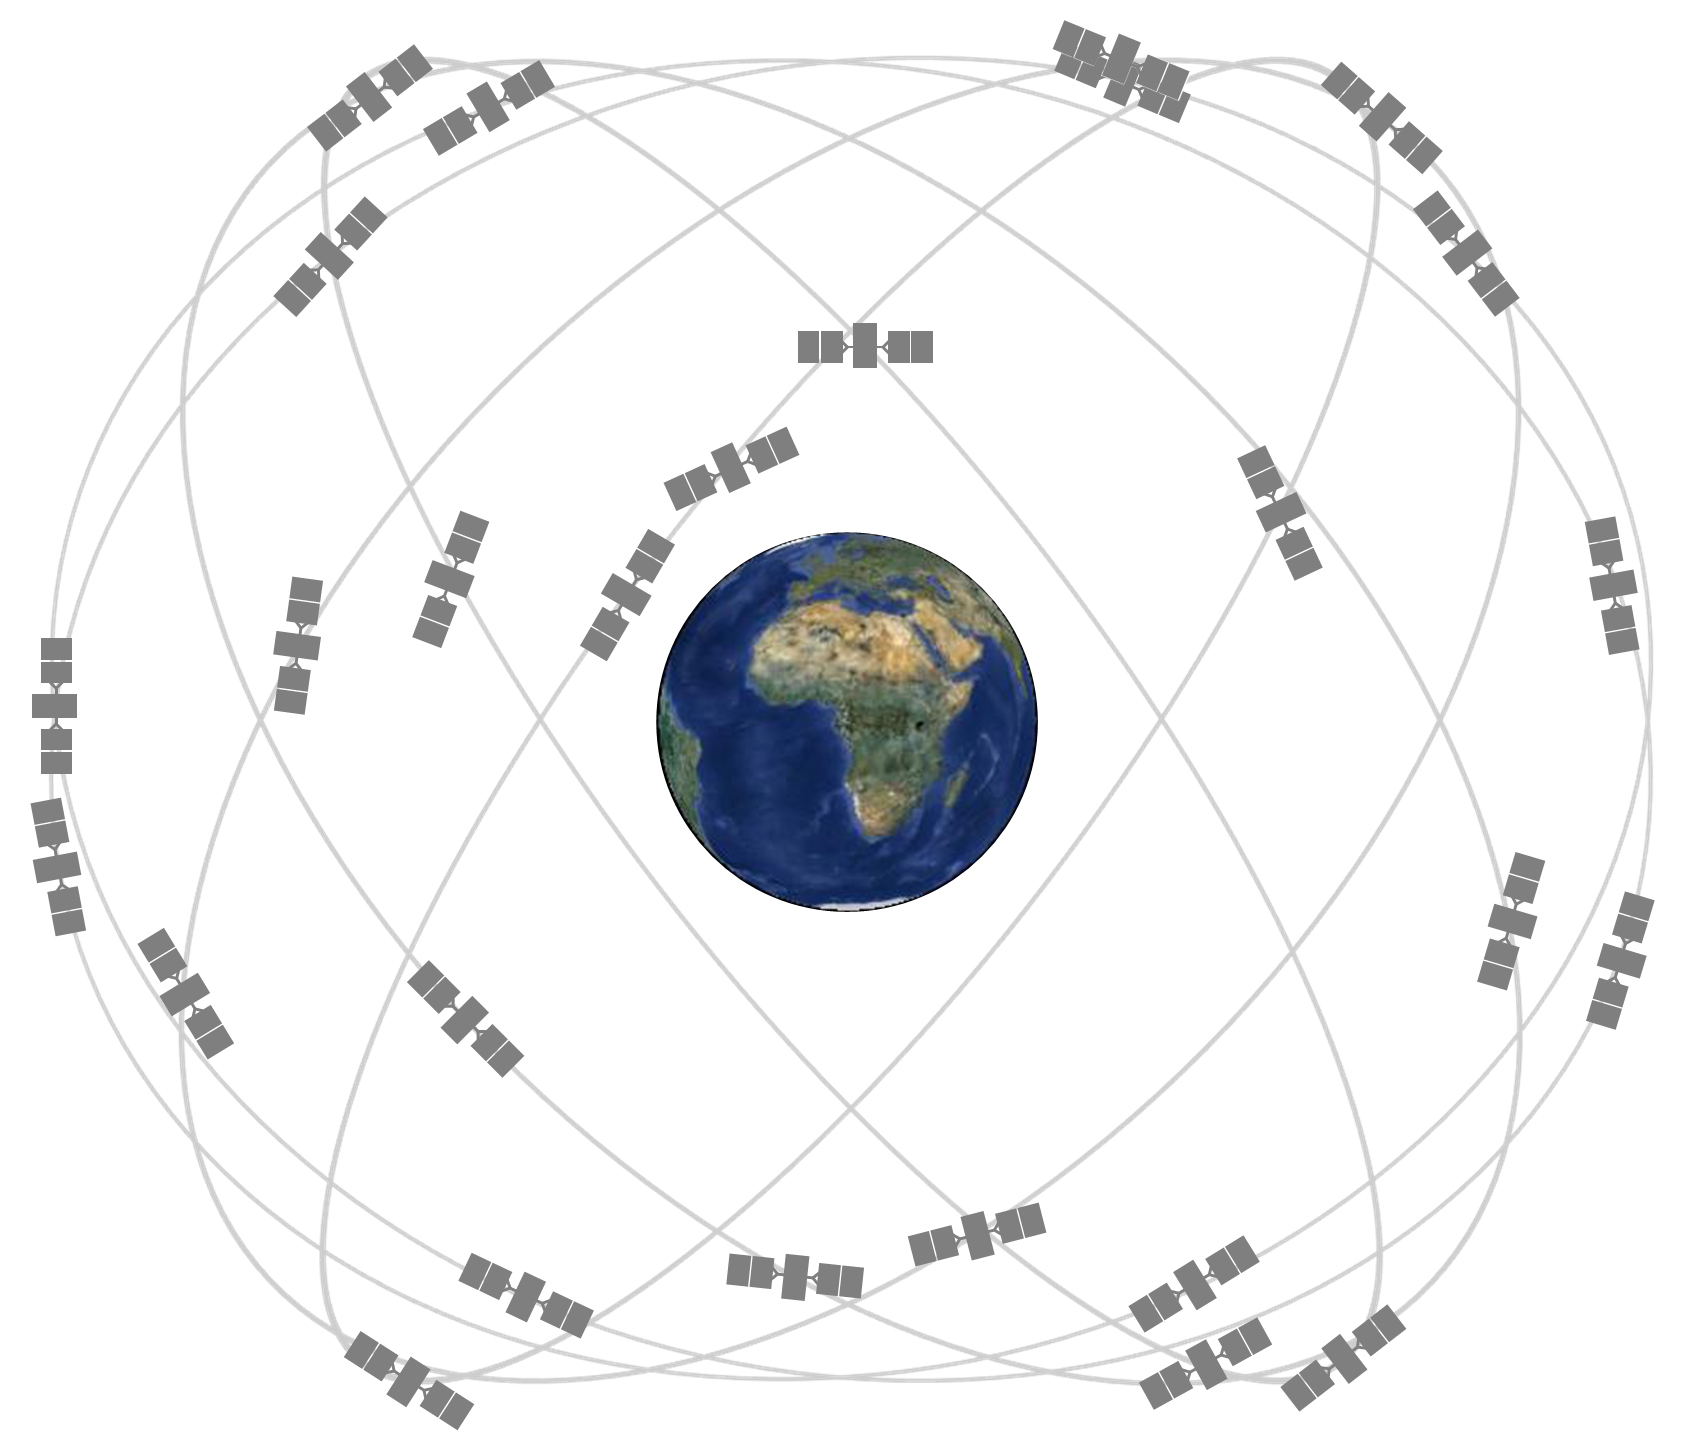
\includegraphics[height=5cm]{images/constellation.jpg}
 \caption{GPS satellite constellation, source: GPS.gov}
 \label{fig:constellation}
\end{figure}

\subsubsection{Control Segment}

To ensure an accurate positioning service for GPS users, the satellites have to be constantly monitored and maintained.
This is the job of the Control Segment.
It monitors satellite orbits and time to predict satellite ephemerides and clock parameters.
It then updates the satellite navigation data, which is later sent from the satellite to the user.
If neccesary, the Control Segment can order the satellites to performe maneuvers to maintain a correct orbit or to relocate to another orbit.
The Control Segment comprises of a network of ground based stations spread arround the globe.
This network is coordinated by the Master Controll Station in the U.S. state of Colorado.

\subsubsection{User Segment}

The User Segment is where the satellite signals are picked up and the position of the user is estimated.
Unlike the other segments, the User Segment is not developed by the U.S. Government, apart from military receivers.
The design of civil GPS receivers is left to the market.
The size of those receivers droped dramatically during the lifetime of GPS from the size of a backpack, to the size of a single IC.

\subsection{Reference Frame}

A navigation system needs a common reference frame.
In the case of GPS, this is the World Geodic System 1984 (WGS84).
Most calculations when using GPS are not done using latitude, longitude and altitude, but an earth-centered, earth-fixed (ECEF) reference frame shown in figure \ref{fig:wgs84}.
In the case of WGS84, the origin is at the mass center of the earth and a position is given with XYZ coordinates.
The X-axis goes through the equator at the longitude of Greenwich.
The Z-axis goes through the north pole and the Y-axis has a right angle to both of the other axes.

\begin{figure}[ht]
 \centering
 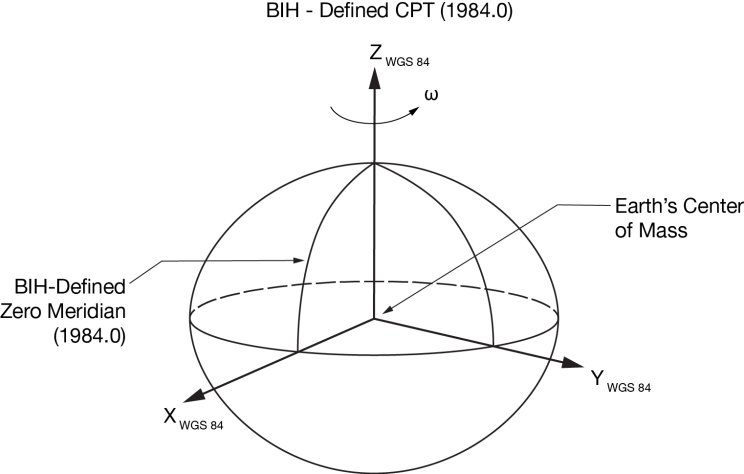
\includegraphics[width=0.7\textwidth]{images/WGS84.png}
 \caption{Definition of the WGS84 reference frame, source: NovAtel.com}
 \label{fig:wgs84}
\end{figure}


\subsection{Functional Principle}

GPS works with the principle of trilateration.
For this method of postitoning, the distance to three known lacations is needed to calculate the own position in three dimensions.
This works with basic vector geometry.
The euclidean distance between two points in three-dimensional space can be calculated with equation \ref{eq:euclidean_dist}.

\begin{equation}
 r^{(k)} = \sqrt{(x^{(k)} - x)^2 + (y^{(k)} - y)^2 + (z^{(k)} - z)^2} = \lvert\lvert \textbf{x}^{(k)} - \textbf{x} \rvert\rvert		\label{eq:euclidean_dist}
\end{equation}

For GPS, the two points are the user position $[x, y, z]$ and the satellite position $[x^{(k)}, y^{(k)}, z^{(k)}]$ and the true distance between them is called $r^{(k)}$ as shown in figure \ref{fig:triangulation}.
The satellites are distinguished with the superscript $^{(k)}$ where k stands for the k-th satellite in view.
In theory, with the position and distance of three satellites, a system of equations could be solved for the three variables of the user position $[x, y, z]$.
But in practice, a gps receiver needs at least four satellites to estimate its position.
This is because a fourth variable needs to be estimated called $\delta t_u$.
This is the difference between GPS time and receiver time.

\begin{figure}[ht]
 \centering
 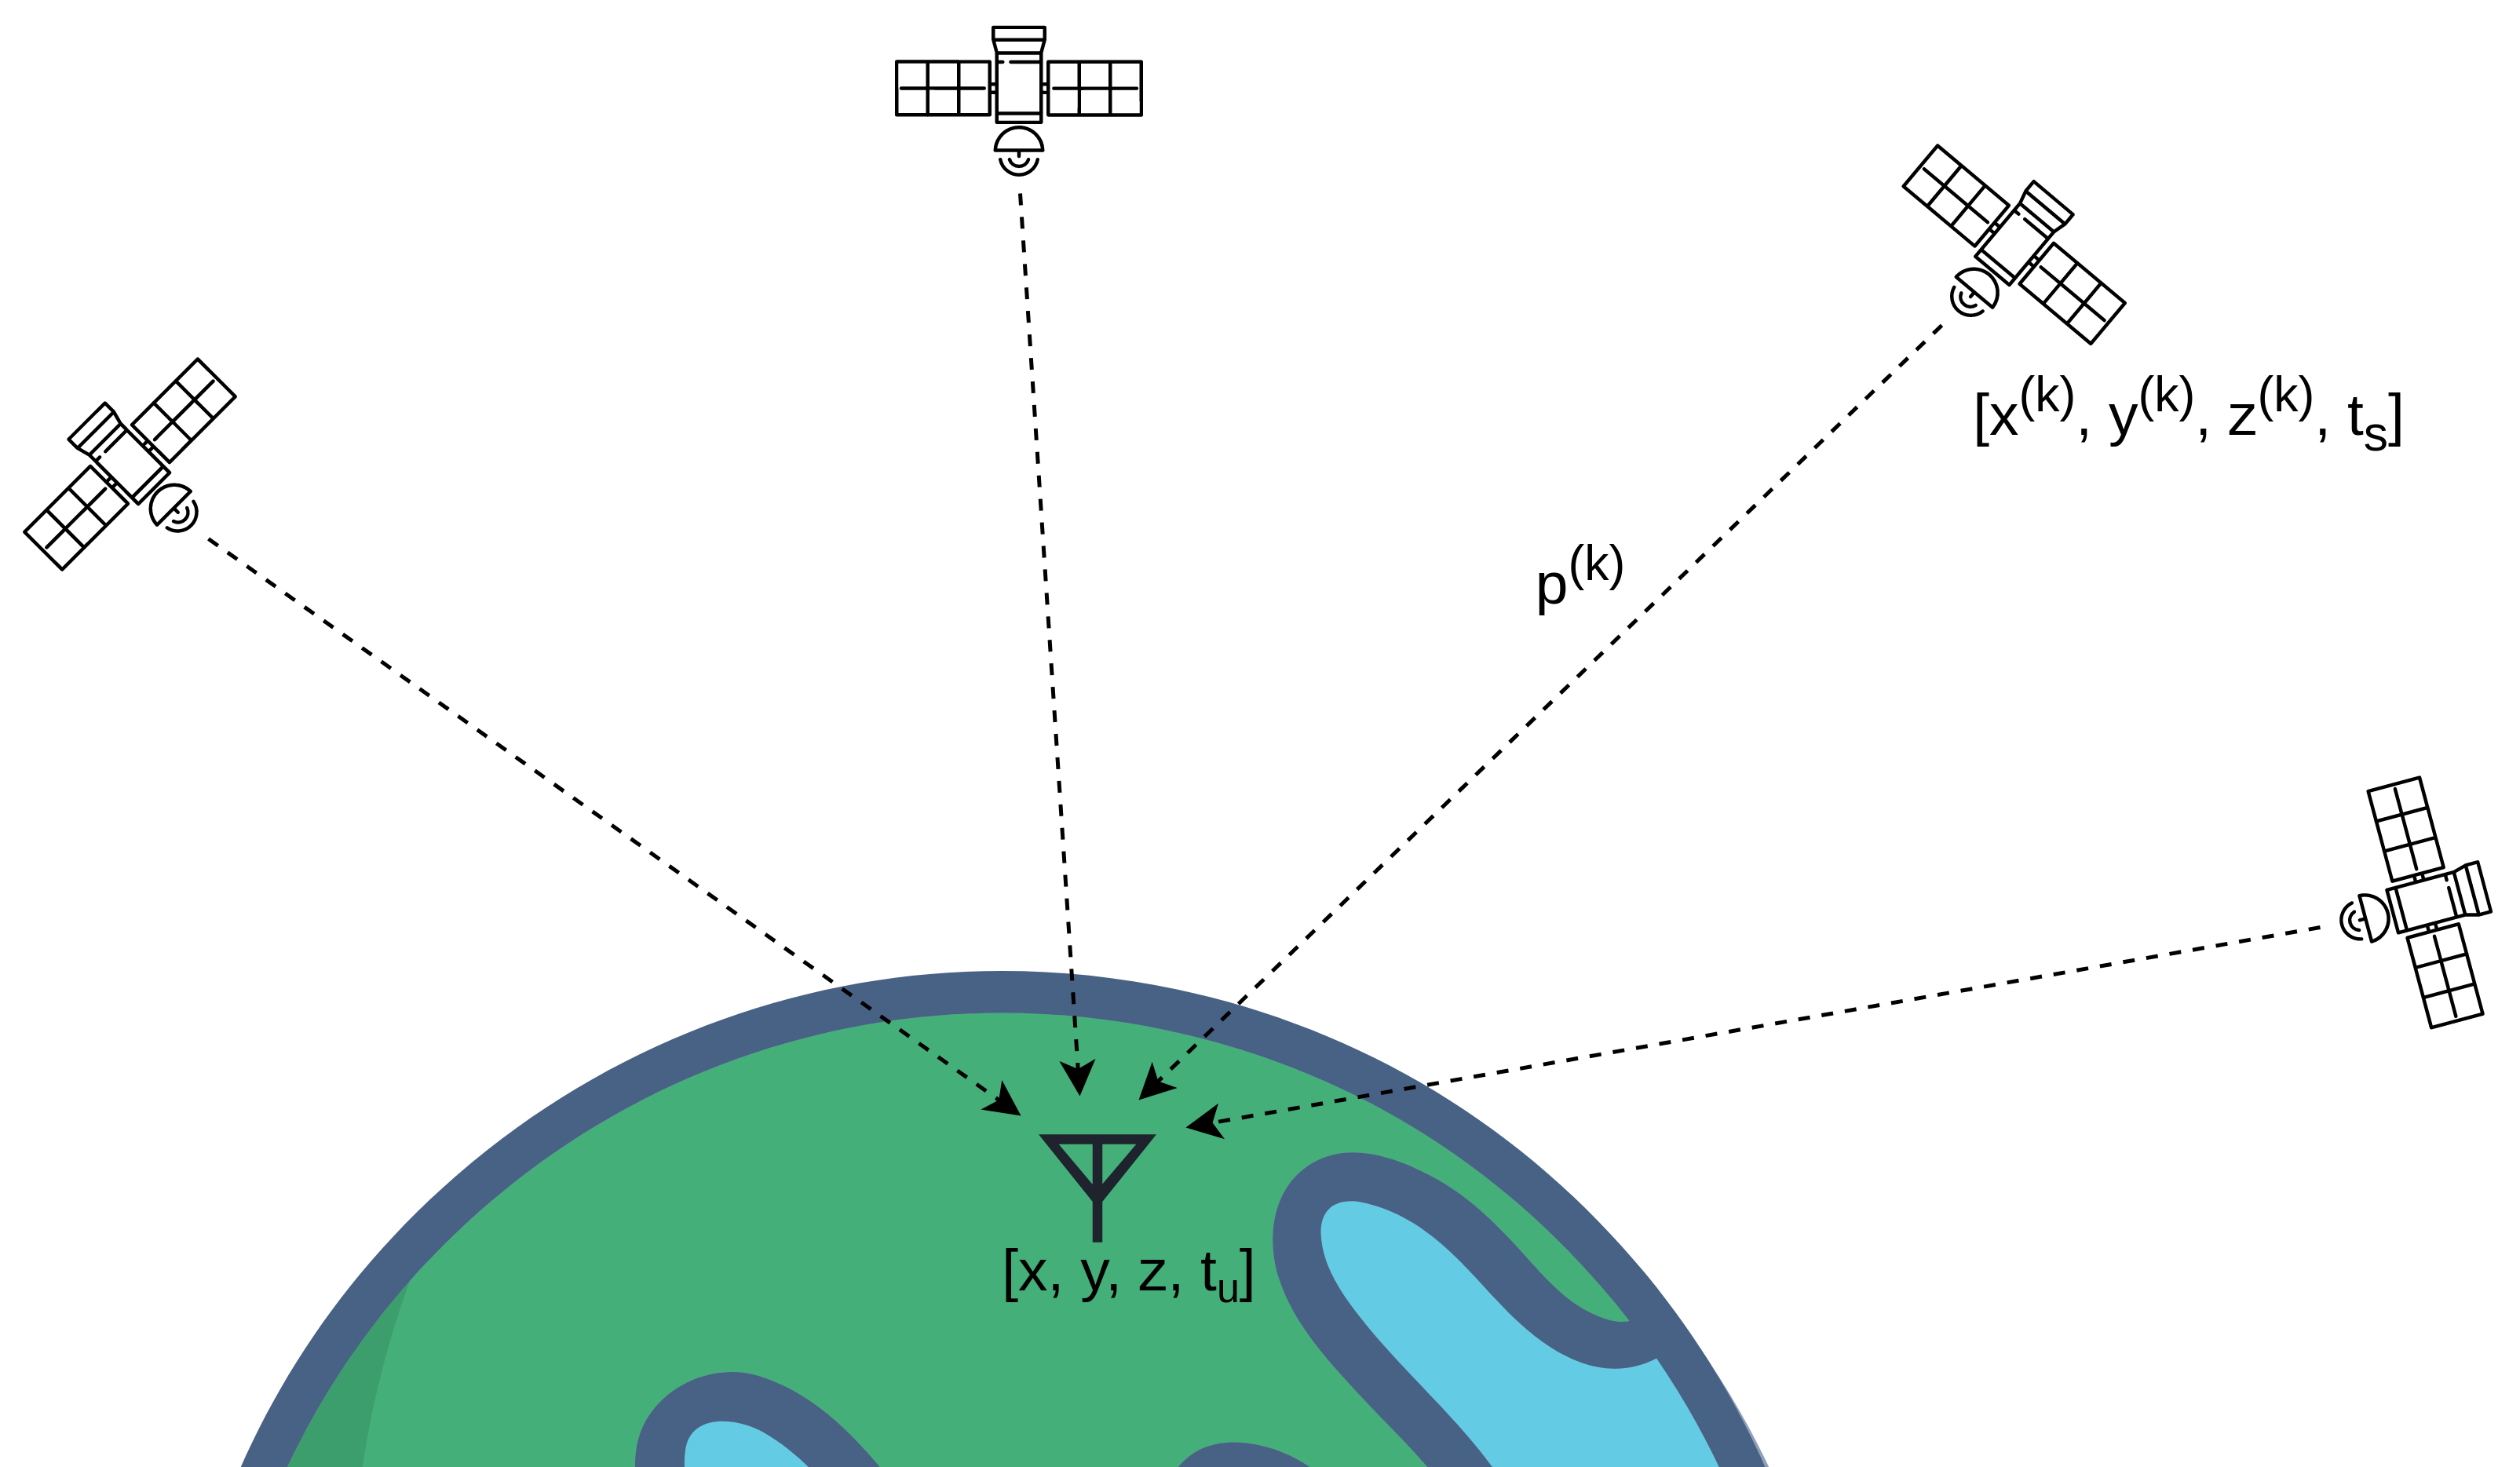
\includegraphics[width=0.8\textwidth]{images/Position_Estimation.png}
 \caption{GPS triangulation}
 \label{fig:triangulation}
\end{figure}

GPS uses the propagation time of radio waves to determine the distance between satellite and user.
The measured transmision time is multiplied by the speed of light to get the distance in meters.
This is not the true distance $r^{(k)}$.
Insted, the so called pseudorange $\rho^{(k)}$ is measured, which contains the true range and a set of errors.
The relation is shown in equation \ref{eq:pseudorange}.
The pseudorange contains the clock errors $c[\delta t_u - \delta t^{(k)}]$ and the atmospheric errors $I^{(k)} + T^{(k)}$.
Those errors can be modeled and estimated to correct the pseudorange.
All the errors that can not be modeled are combined in the term $\varepsilon^{(k)}$.
What these errors mean is closer explained in section \ref{sec:error_sources}.

\begin{equation}
 \rho^{(k)} = r^{(k)} + c[\delta t_u - \delta t^{(k)}] + I^{(k)} + T^{(k)} + \varepsilon^{(k)}		\label{eq:pseudorange}
\end{equation}

Important here is the user clock error $\delta t_u$.
The reason for this error is the inaccurate clock in the receiver.
The satellites have atomic clocks which are synchorinized to GPS time.
It is not feasable to build an atomic clocks into every receiver and keep it synchorinized to GPS time.
Insted, the difference between receiver time and GPS time is estimatet with the measurement of a fourth satellite.
This is possible because the user clock error is common in the pseudoranges from all satellites.
The estimation of the four variables $[x, y, z, \delta t_u]$ is either done iteratively with the Least Square method or with a Kalman Filter.

\subsection{Signals}

A GPS receiver can work with only the information included in the signals from the satellites.
This means the information for distance and satellite position have to be transmitted with those signals.
GPS solves this problem with a three-layered signals like the one in figure \ref{fig:signal_structure}.

\begin{figure}[ht]
 \centering
 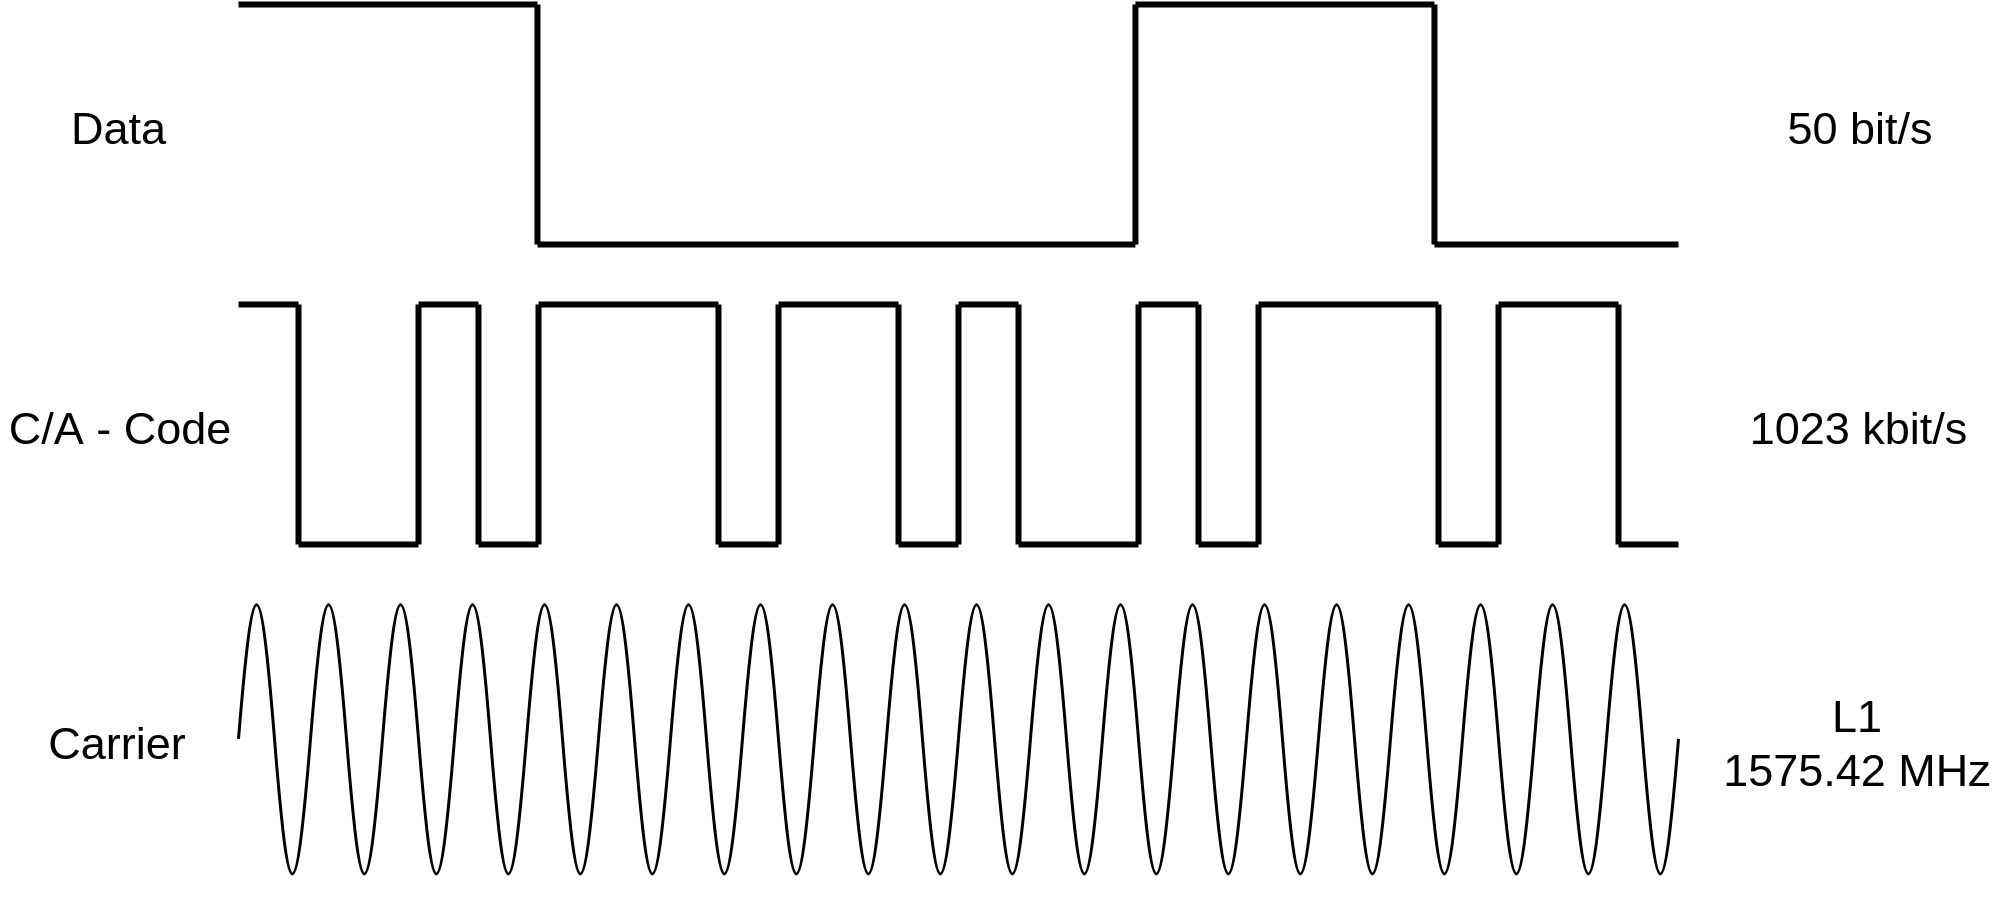
\includegraphics[width=0.8\textwidth]{images/Signal_Structure.png}
 \caption{C/A-code signal structure (not to scale)}
 \label{fig:signal_structure}
\end{figure}

The carrier is a sinusoidal signal in the L band.
Most civil GPS receivers work with the L1 signal at 1575.42 MHz.
GPS satellites also send on L2 at 1227.6 MHz and newer satellites on L5 at 1176.45 MHz too.
A variety of civil and encrypted military signals are modulated onto those carriers.
The main signal for civil applications is the C/A-code on L1.
It consists the C/A-code itself and a data stream.
The C/A-code and the data stream are both binary sequences.
They are first XORed together and then modulated onto the carrier using Binary Phase Shift Keying (BPSK).
This process of XORing is equal to the spreading of the spectrum with the pseudorandom C/A-code sequence.

The C/A-code is a sequence of 1023 bits, which repeats every millisecond and is unique to each satellite.
The lenght of each bit, or chip in this context, is about 1 $\mu s$.
Besides the spreading and despreading of the spectrum, this code is used to measure the signal transmission time.
The received signal is demodulated and correlated with local copies of the C/A-codes on separate channels.
The local copy is shifted in time until an autocorrelation peak emerges.

The actual data transmitted with only 50bit/s is the navigation message.
It contains information about the satellites time, orbit, clock correction and ionospheric correction.
The obit data is called ephemeris.
With it, the position of the satellite can be calculated.
The satellites clock and ionospheric corrections are used to correct the pseudorange for the terms $\delta t^{(k)}$ and $I^{(k)}$.

The transmitted GPS time with the current bit location in the navigation message frame and the delay from the code correlation combined make up the pseudorange measurement.

\subsection{Performance}

To evaluate the performance of GPS, a number of metrics can be used.
The most prominent one is of course the accuracy.
This was already addressed in section \ref{sec:requirements}, where the requirements were defined.
Accuracy can be explained with the two errors variance and bias.
In GPS, the two errors are often not given separately when the accuracy of the whole system is described.
Accuracy simply describes how close the measurement matches the real position.
The two most used metrics to describe GPS postitoning accuracy are the 95th precentile and the RMS error.
The 95th precentile describes the value in meters, where 95 \% of errors are smaller and 5 \% are larger.
The RMS error equals the variance of 1 $\sigma$, as long as the mean error is zero.
A mean error is a bias, that is considered in the RMS error but does not impact the variance.
The RMS error is calculated with:
\begin{equation}
 Error_{RMS} = \sqrt{\frac{\sum\limits_{i=1}^n \lvert\lvert \textbf{x}_{real} - \textbf{x}_{meas} \rvert\rvert^2}{n}}
\end{equation}

The error can be further divided into horizontal and vertical error.
The GPS Standard Positioning Service (SPS) Performance Standard defines an average $\leq$ 9 m for 95 \% horizontal error and a $\leq$ 15 m for 95 \% vertical error \cite{SPS_Performance}.

Other than accuracy, availability and integrity are two other important metrics.
The availability is the likelihood a user anywhere on earth can get a GPS fix.
The GPS SPS Performance Standard defines a $\geq$ 99 \% locational availability \cite{SPS_Performance}.
Integrity is how trustworthy the information of the system is.
This is especially important for safety-of-life applications like airplane navigation.
GPS constantly monitors itself and informs the user if the data does not meet the requirements.
This is done with satellite self-monitoring, cross-monitoring between satellites, and ground based monitoring. \cite{misra2011global}


\section{Error Sources}\label{sec:error_sources}

The amount of error in the GPS position is determined by two Factors.
The reason there is a position error at all is the unmodeled error in the pseudoranges called User Range Error (URE).
This error is further divided into three groups of errors depending on where they occure.
Errors in the satellites state are called satellite errors.
Errors that occure in the signal path from the satellite to the receiver are called atmospheric errors.
Finally, errors that are caused by unprecise measurenents of the signals by the receiver are called measurement errors.
All three types are discussed later in this section.

The other factor is the satellite geometry.
It determines how much the URE impacts the position accuracy.
An optimal geometry would be stellites evenly distributed in all three dimensions.
This is not possible because a receiver on the surface of the earth can not receive signals from satellites blocked by the earth.
A metric to determine the geometry quality is the Dilution of Precision (DOP).
Different versions of DOP can be determined like the Horizontal DOP (HDOP), Vertical DOP (VDOP), 3-D Position DOP (PDOP) and Time DOP (TDOP).
The RMS position error can then be calculated with the standard deviation of the URE $\sigma_{URE}$ multiplied with the corresponding DOP.
For example, the horizontal RMS position error can be calcuated with:
\begin{equation}
 Horizontal \text{ } Error_{RMS} = \sigma_{URE} \cdot HDOP
\end{equation}

\subsection{Satellite Errors}

\begin{minipage}{0.6\textwidth}
  GPS satellites broadcast a navigation message with 50 bps which includes orbital parameters to calculate their position.
  Orbital parameters of a GPS satellite are called ephemeris. 
  Those parameters are estimated and uploaded to the satellites by the control segment.
  The difference between the estimated position and the real satellite position is called ephemeris error.
  
  The other satellite error comes from an inaccurate satellite clock.
  Although GPS satellites have atomic clocks, they can never be perfectly alligned with GPS time.
  That is why the control segment also estimates a clock offset for each satellit, which is also broadcasted with the navigation message.
  This correction apperars in the pseudorange equation \ref{eq:pseudorange} as $\delta t^{(k)}$.
  
  The remaining satellite errors after the pseudorange correction are the errors in the ephemeris estimation and satellite clock offset estimation.
  They are determined by how accurate the control segment can determine the position and time of each satellite.
\end{minipage}
\hfill
\begin{minipage}{0.38\textwidth}
 \flushright
 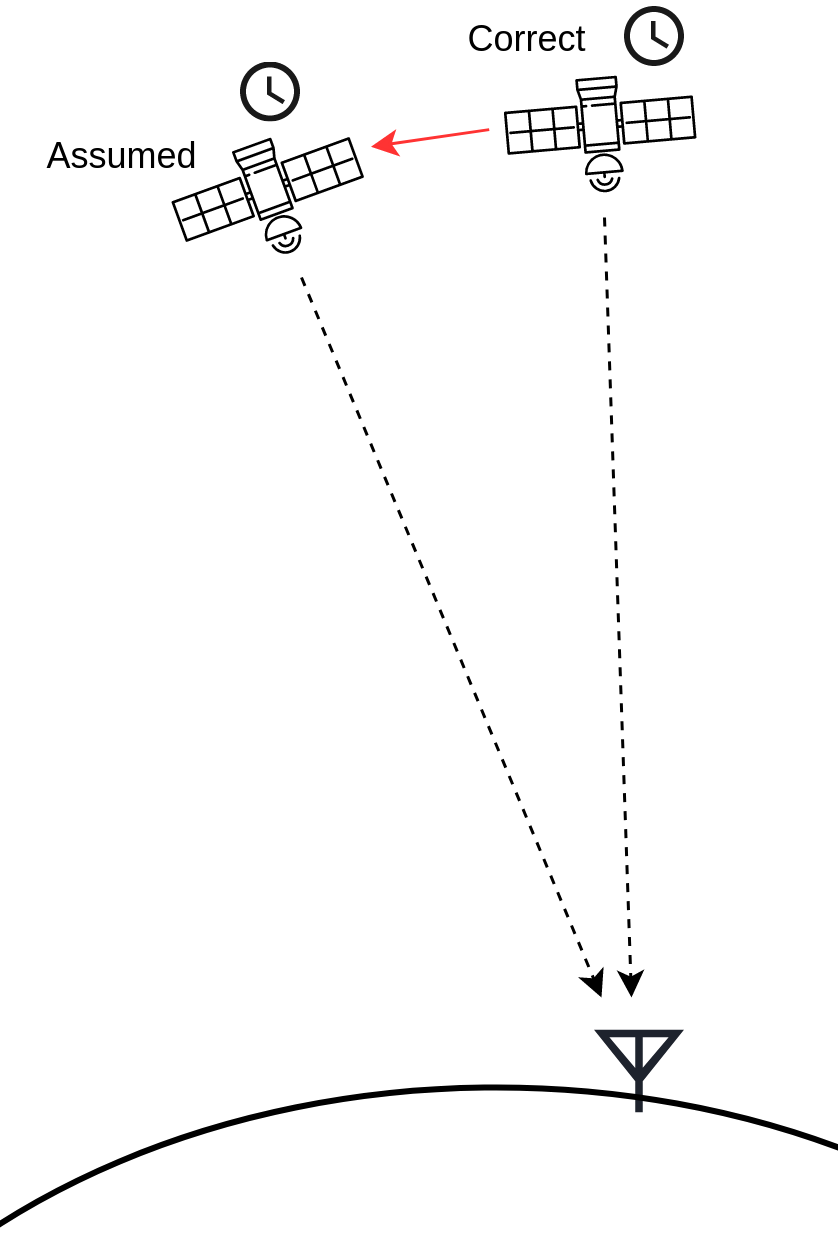
\includegraphics[width=\textwidth]{images/Satellite_Errors.png}
 \captionof{figure}{Ephemeris and time satellite errors}
\end{minipage}

\subsection{Atmospheric Errors}

\begin{minipage}{0.6\textwidth}
  The orbits of GPS satellites are at about 20'200 km above the earths surface.
  To get the pseudorange, the signal transmission time is multiplied by the speed of light.
  This implies that the signal travels through only vacuum.
  In reality, this is not entirely accurate.
  On the way from the satellite to the receiver, the signal has to pass trough large parts of earths atmosphere.
  Especially two atmospheric layers influence the propagation time of the signal.
  The first one is the ionosphere between about 50 km and 1000 km.
  It consists of ionized gases.
  The intensity of the ionization depends mainly on the sun's activity and the day/night cycle.
  The ammount of ionization determines the delay added to the transmision time by the ionosphere.
  The zenith delay in meters varies from 1 m up to 36 m. 
  It can increase by a factor of 3 with a lower elevation of the satellite.
  The ionosphereic delay can be modeled to a certain extent with the current space weather and appers in the pseudorange equation \ref{eq:pseudorange} as $I^{(k)}$.
\end{minipage}
\hfill
\begin{minipage}{0.38\textwidth}
 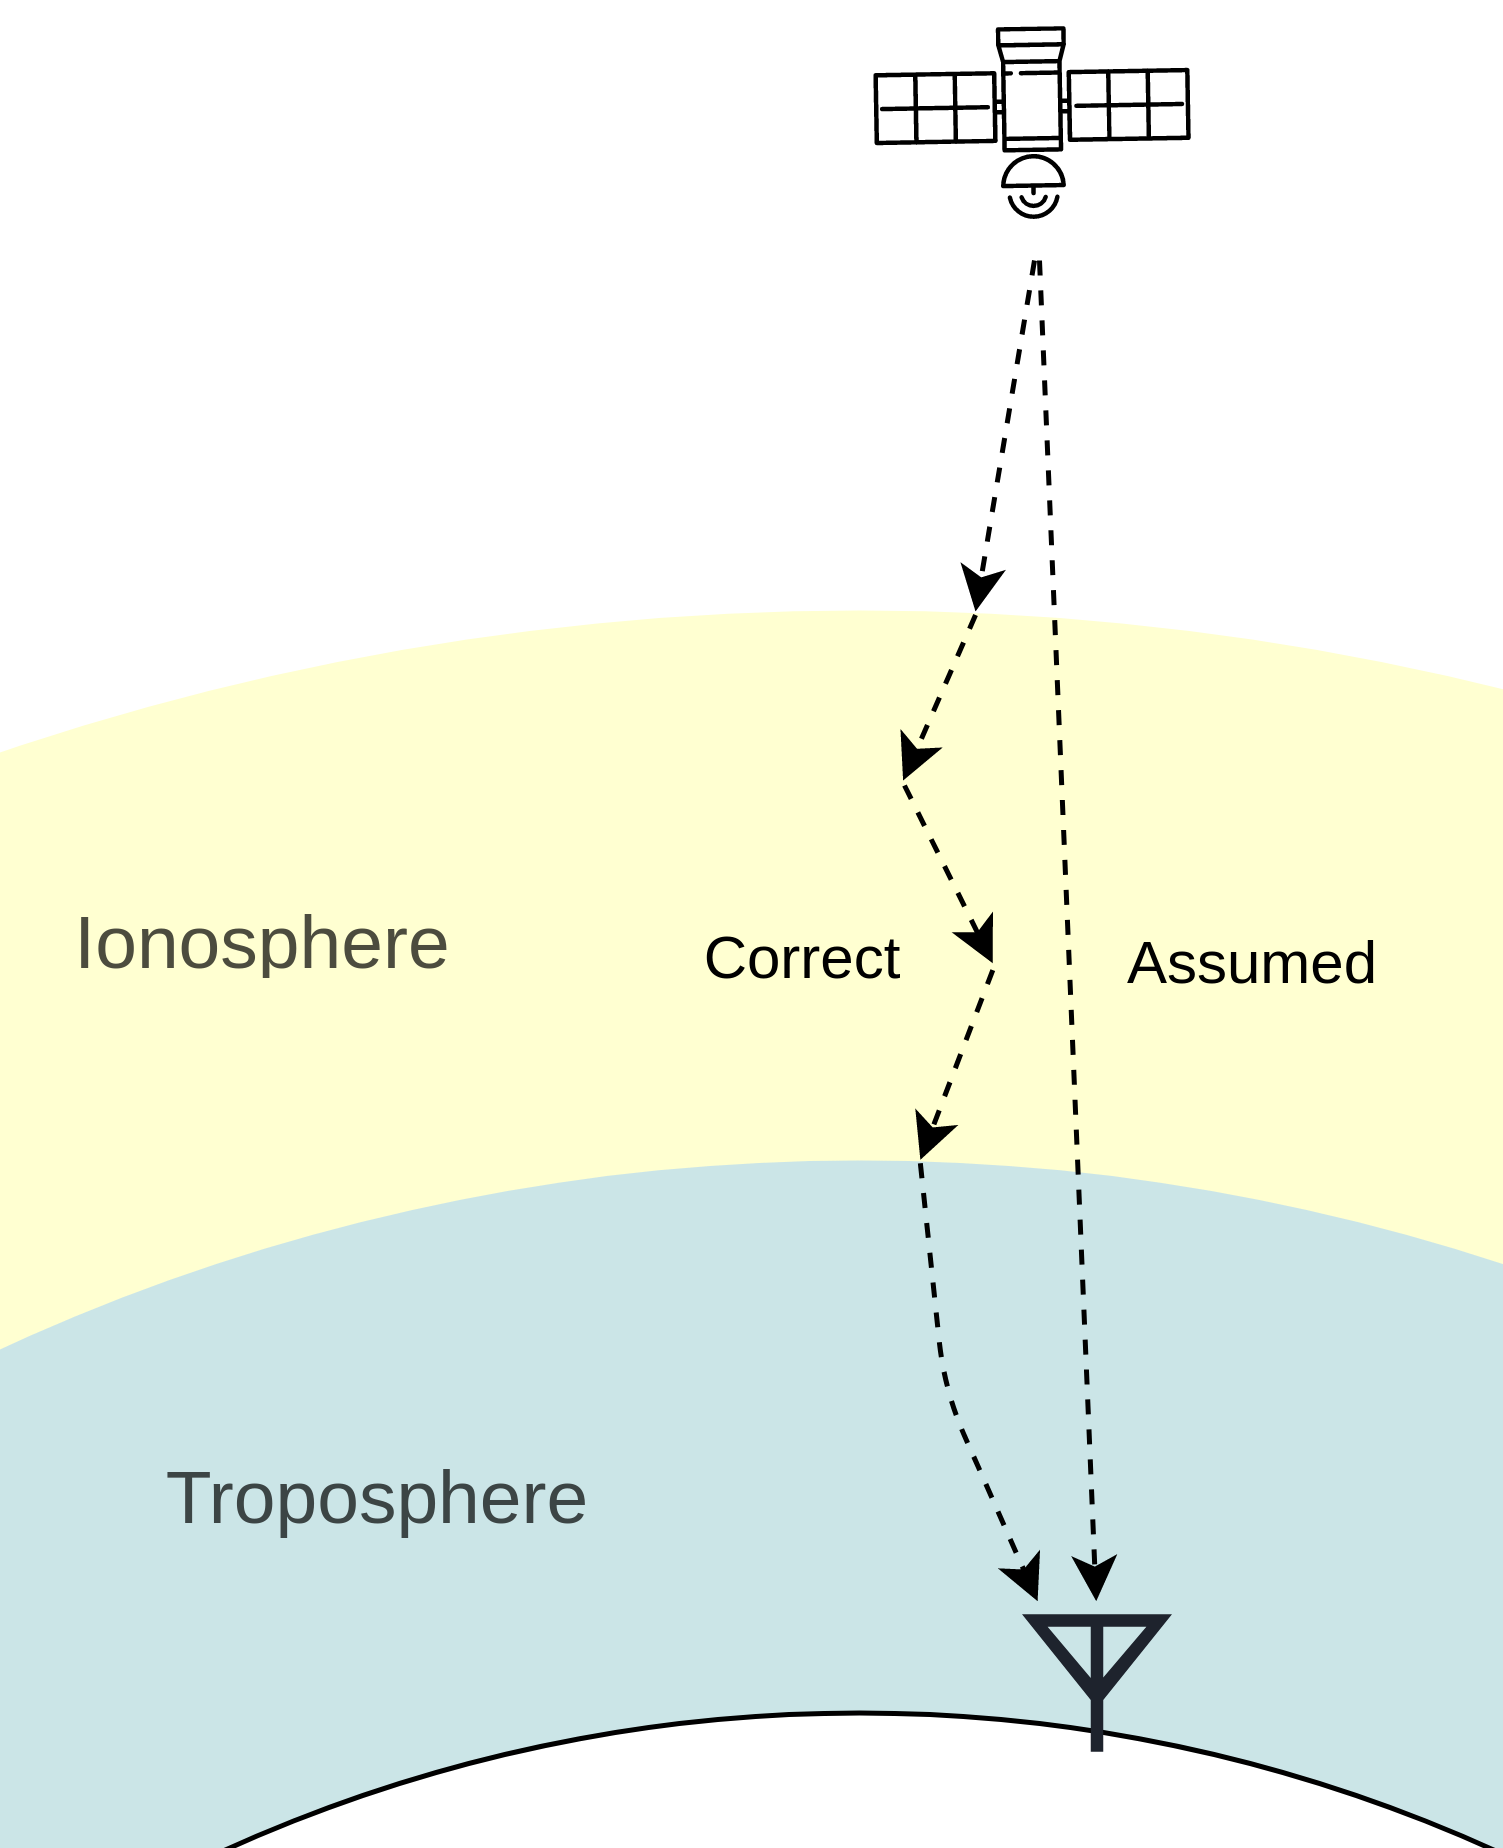
\includegraphics[width=\textwidth]{images/Atmospheric_Errors.png}
 \captionof{figure}{Ionosphereic and tropospheric errors}
\end{minipage}

The other important layer is the troposphere.
It is the lowest part of the atmosphere and extends from the ground to about 9-16 km depending on the latitude.
The troposphere contains three-quarters of the gaseous mass and all of the water vapor of the atmosphere.
This matter slows the signal down and results in a zenith delay of 2.3-2.6 m at sea level.
With a lower elevation of the satellite, the delay can increas by a factor of 10.
It can be modeled with the atmospheric humidity and pressure, and is fairly stable because the biggest influence has the gaseous mass, which does not change much over time.
The term for tropospheric delay in the pesudorange equation \ref{eq:pseudorange} is $T^{(k)}$.

\subsection{Measurement Errors}

Unlike the previous errors, measurement errors depend on factors like signal power, code structure and receiver design.
Multipath is a problem most wireless communication systems have.
The signal is refelcted by surfaces and arrives at the receiver miltiple times at different times.
Normally, there is a main signal from the line-of-sight path, and weaker, delayed versions of the signal.
The influence on the measured range depends on the strength and delay of the reflected signal.

Receiver noise is a general term for noise added by the antenna, amplifiers, cables and the receiver.
RF radiation noise which is picked up by the antenna also adds to the effect of receiver noise.
The strength of the receiver noise relative to the GPS signal determines the signal-to-noise ratio.
A low signal-to-noise ratio results in a tracking error of the GPS code, which in turn directly impacts the pseudorange measurement.

None of those errors can be modeled, so they are included in the term $\varepsilon^{(k)}$ in the pseudorange equation \ref{eq:pseudorange}. \cite{misra2011global}

\begin{minipage}{0.45\textwidth}
 \flushleft
 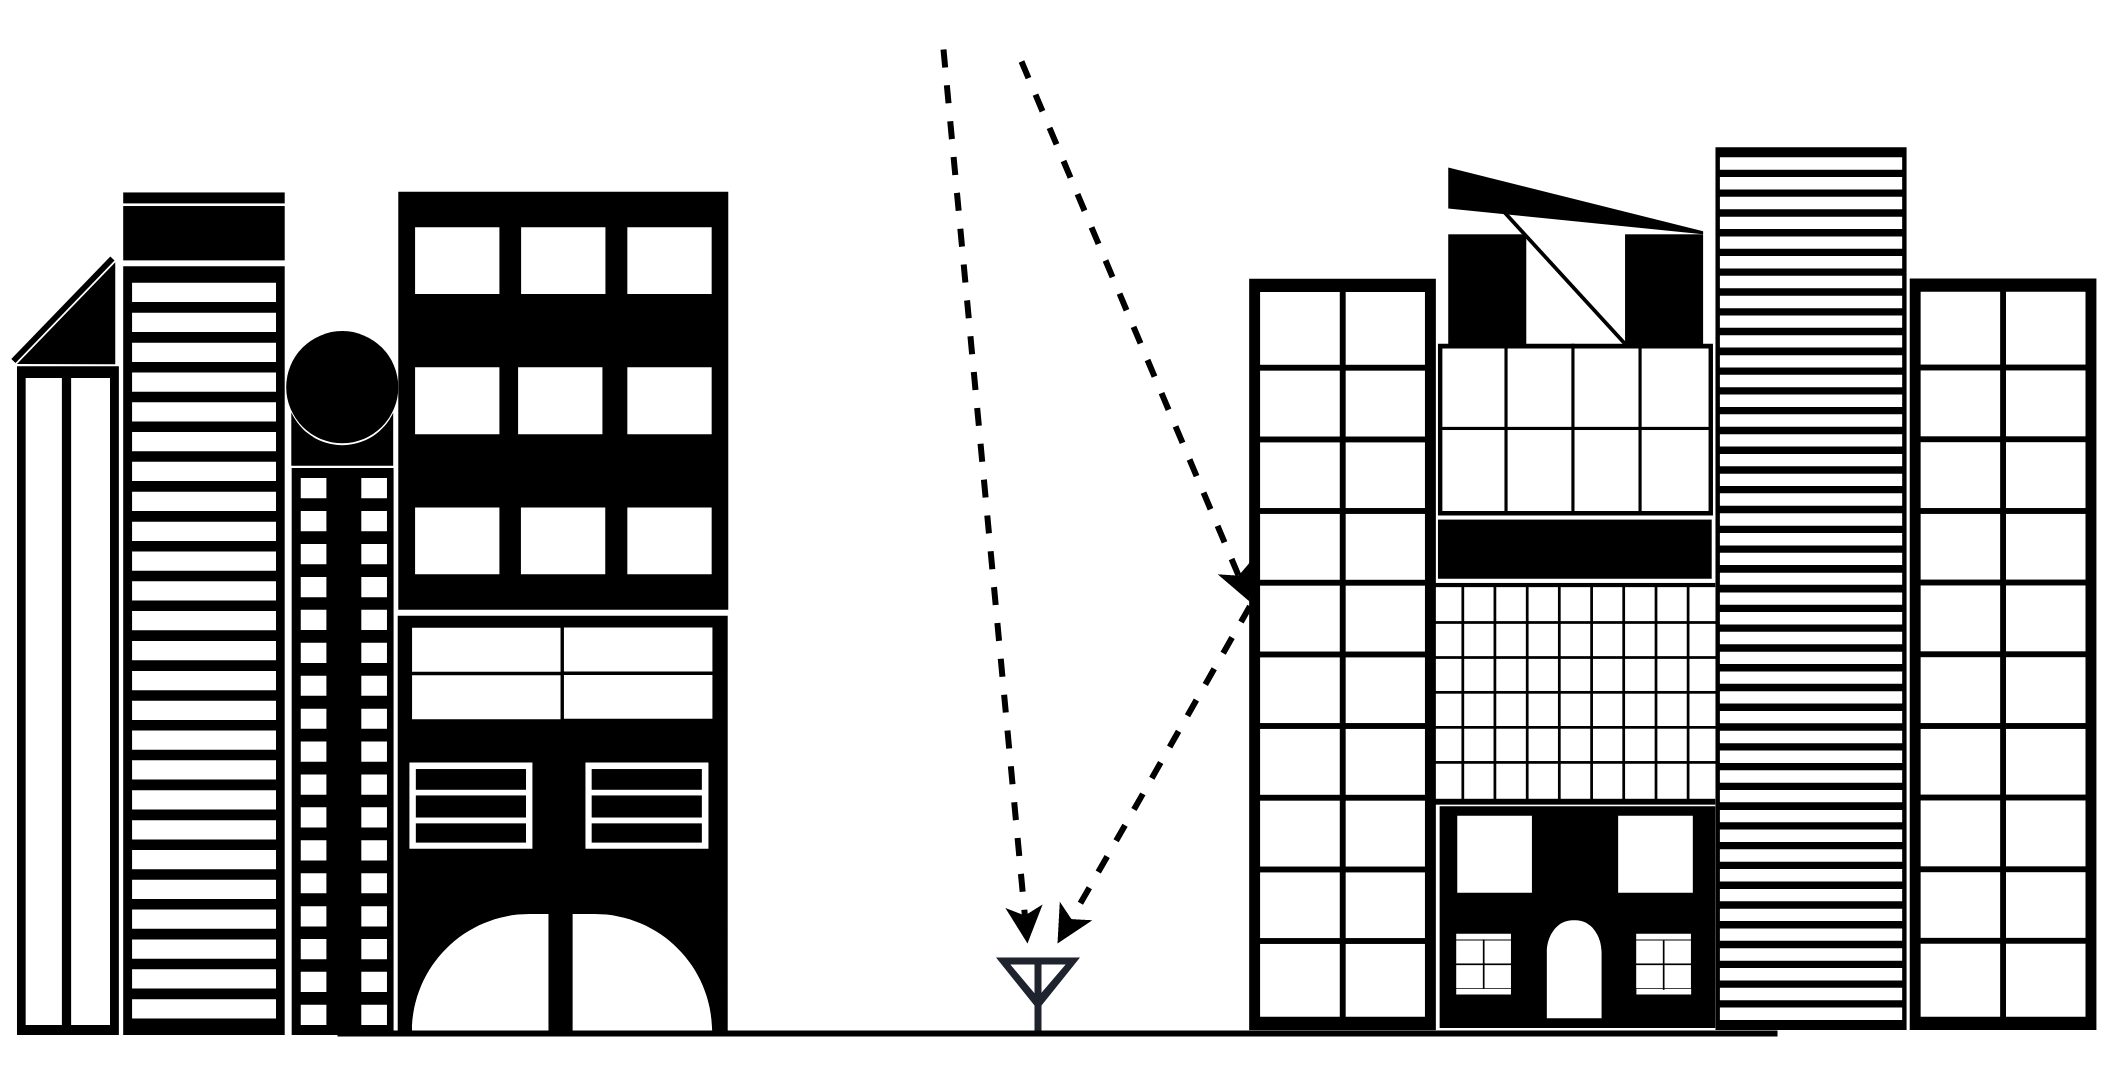
\includegraphics[width=\textwidth]{images/Multipath.png}
 \captionof{figure}{Multipath in an urban canyon}
\end{minipage}
\hfill
\begin{minipage}{0.45\textwidth}
 \flushright
 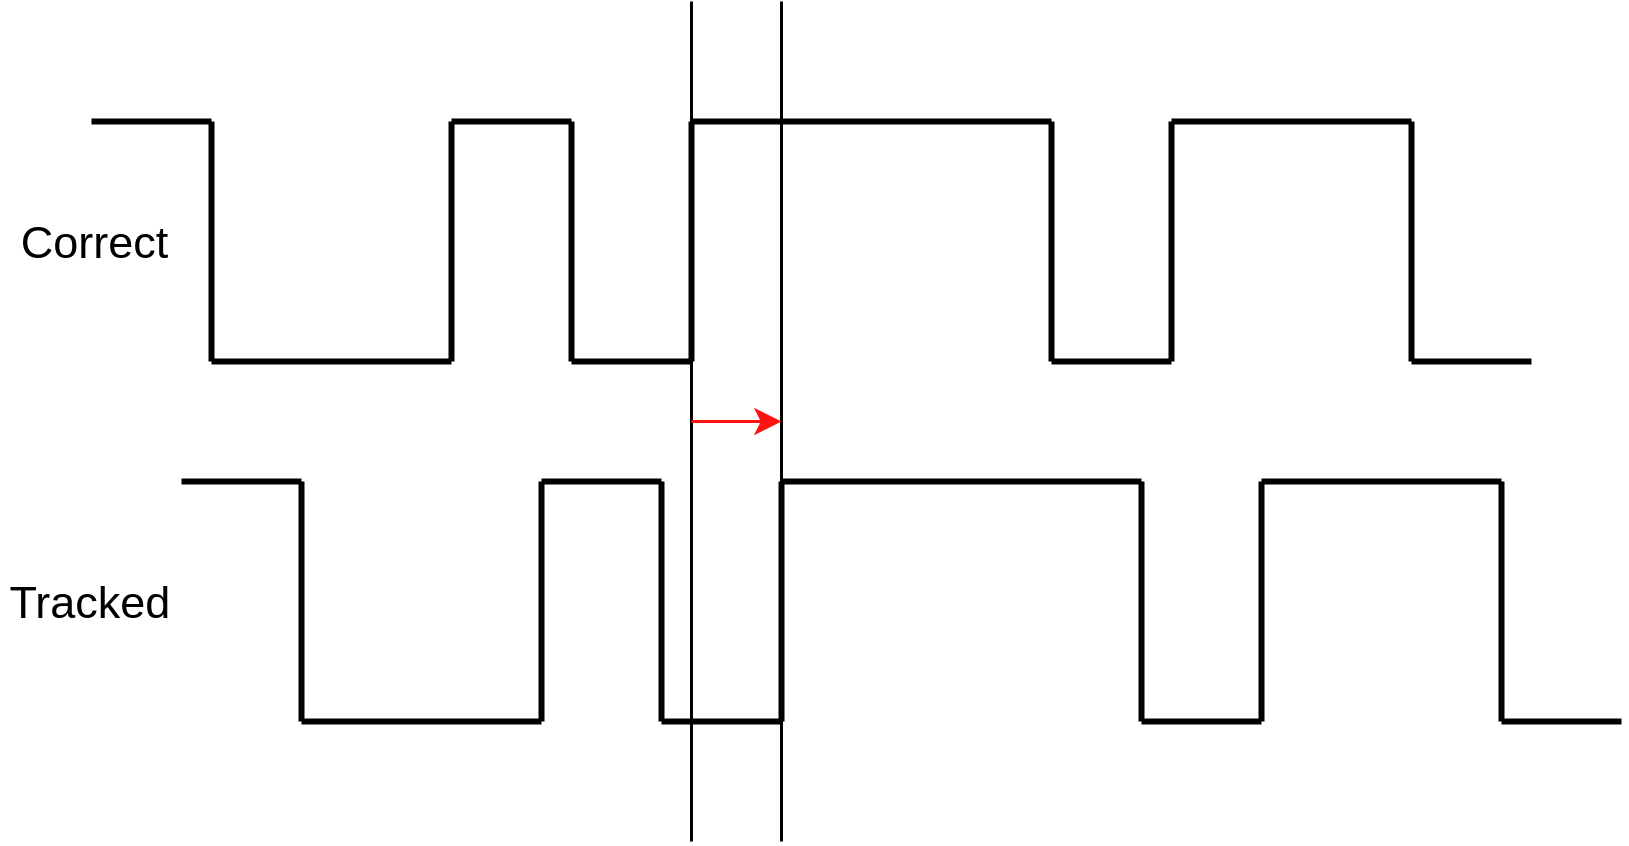
\includegraphics[width=\textwidth]{images/Receiver_Noise.png}
 \captionof{figure}{Tracking error caused by receiver noise}
\end{minipage}


 
 \chapter{Accuracy Enhancement Systems}


\section{Carrier-Phase Measurements}

\section{Differential GPS}

\section{Real Time Kinematic}

\section{Satellite-Based Augmentation Systems (SBAS)}

\section{Summary}
 
 \chapter{Differential GPS concept for a sounding rocket}

\subsubsection{Setup:}
\begin{itemize}
 \item Two M8T modules in the nosecone and one at the ground station.
 
 \item RF-uplink from ground station to rocket.
\end{itemize}


\subsubsection{Procedure:}
\begin{itemize}
 \item Ground station averages position measurements over a longer time to get reference position. 
 This might not be the exact position, but this only results in a constant bias in the rockets absolute position. 
 Reference position stays fixed when sending of differential correntions starts.
 
 \item Ground station calculates distance to each visible GPS satellite from reference position and ephemeris data.
 
 \item The differnce between the calculated distance and the measuren pseudorange is calculated for each satellite.
 
 \item RTCM 2.3 meassage 1 and 3 are created with the pseudorenge corrections.
 
 \item The RTCM messages are sent to the rocket over the RF-link. 
 The update rate of the corrections could be about 1Hz.
 
 \item On the rocket, the messages are fed into the UART interface of the GPS receiver which includes them in the position estimation.
 
 \item Tropospheric corrections could be added to the pseudorange corrections at the ground station or in the rocket.
 
 \item The first correction is sent when the rocket is still on the launch pad.
 One or more corrected measurements at the launch pad serve as the zero point of the trajectory.
 
 \item The position estimations during the flight can be differnced with the launch pad zero point to get the relative position to the launch pad.
 With this the reference position bias cancels out.
 For the rocket controll and the post processing, the relative position to the launchpad is more relevant.
 The absolute position, where the reference positon bias is still present, is only needed for the recovery of the rocket where accuracy is not as important.
\end{itemize}
 
 \chapter{Implementation}
 
 \chapter{Testing}

The implementation described in the previous chapter now has to be tested.
The testing should show if the implemented system produces the required output.
Testing of single parts of the system like the interface from the application to the GPS receiver or the calculation of satellite positions is not the focus here.
The tests described are on the level of the whole system.
Multiple accuracy tests were planned to test different factors that could impact the system.
Most tests were planned to determine how accurate the DGPS system is compared to standard GPS.
Also the influences of the extreme conditiond on a sounding rocket should be determined with these tests as far as possible.
Unfortunately, there was not enough time to conduct all planned tests.
Only static accuracy tests were conducted.
The most representative is described in section \ref{sec:static_accuracy}.


\section{Testing Setup}

The setup to test the system does not differ much from the system described in the implementation chapter.
The difference is that for static accuracy tests, no wireless communication is needed.
The corrections can be sent directy to a second receiver plugged into the laptop which runs the application.
Two receivers are needed for the DGPS, one as reference station and one as user.
Additionally, a receiver has to measure the position without applying the corrections to have a reference to compare the DGPS to.
This setup can be achieved with only two receivers, when the postition output of the reference receiver is used as the uncorrected GPS measurement.

Needed to evaluate the tests are the position estimations with and without applying the corrections, and the PRCs.
The M8T receiver has the ability to log all its output.
It can later be retrieved with the u-blox software u-center.
The logging of the PRCs can be enabled in the DGPS Message Generator application.

Before the logged data can be evaluated, the messages have to be extracted from the bit straem.
A NMEA parser was written in C++ to extact the GxGGA messages and save them to a .csv file.
They contain GPS fix data like UTC time, latitude, longitude and altitude.
The evaluation is done with Matlab scripts that understands the format of the generated .csv files (Appendix \ref{appendix:matlab_code}).

\section{Static Accuracy}\label{sec:static_accuracy}

Static accuracy test means that the user receiver does not move and is at the same position as the reference station.
This test was done at a surveyed location to be able to measure the absolute position error.
The Swiss Federal Office of Topography Swisstopo manages the control points data used for natonal surveying.
Swisstopo makes the data available online in form of a map \cite{Swisstopo}.
The choosen test location is a control point on the Sonnenberg in Kriens.
Its exact position is given in the corresponding file (Appendix \ref{appendix:control_point_sonnenberg}).

\newpage

\subsection{Setup}

The reference coordinates are given in the local swiss reference frame LV95.
They have to be converted to the WGS84 reference frame in ECEF form.
This was done using the REFRAME online tool from Swisstopo.

\begin{figure}[ht]
 \centering
 \includegraphics[width=\textwidth]{images/measurement_kriens_setup.png}
 \caption{Measurement setup on the Sonnenberg in Kriens}
 \label{fig:measurement_kriens_setup}
\end{figure}

The measurement was conducted on the 26. Mai 2018 from 15:15 until 16:15.
The location can be seen in figure \ref{fig:measurement_kriens_setup}.
The control point is marked by a triangle on the manhole cover.
The two antennas were placed about 10 cm apart and 1 meter above the control point.

\newpage

\begin{figure}[ht]
 \centering
 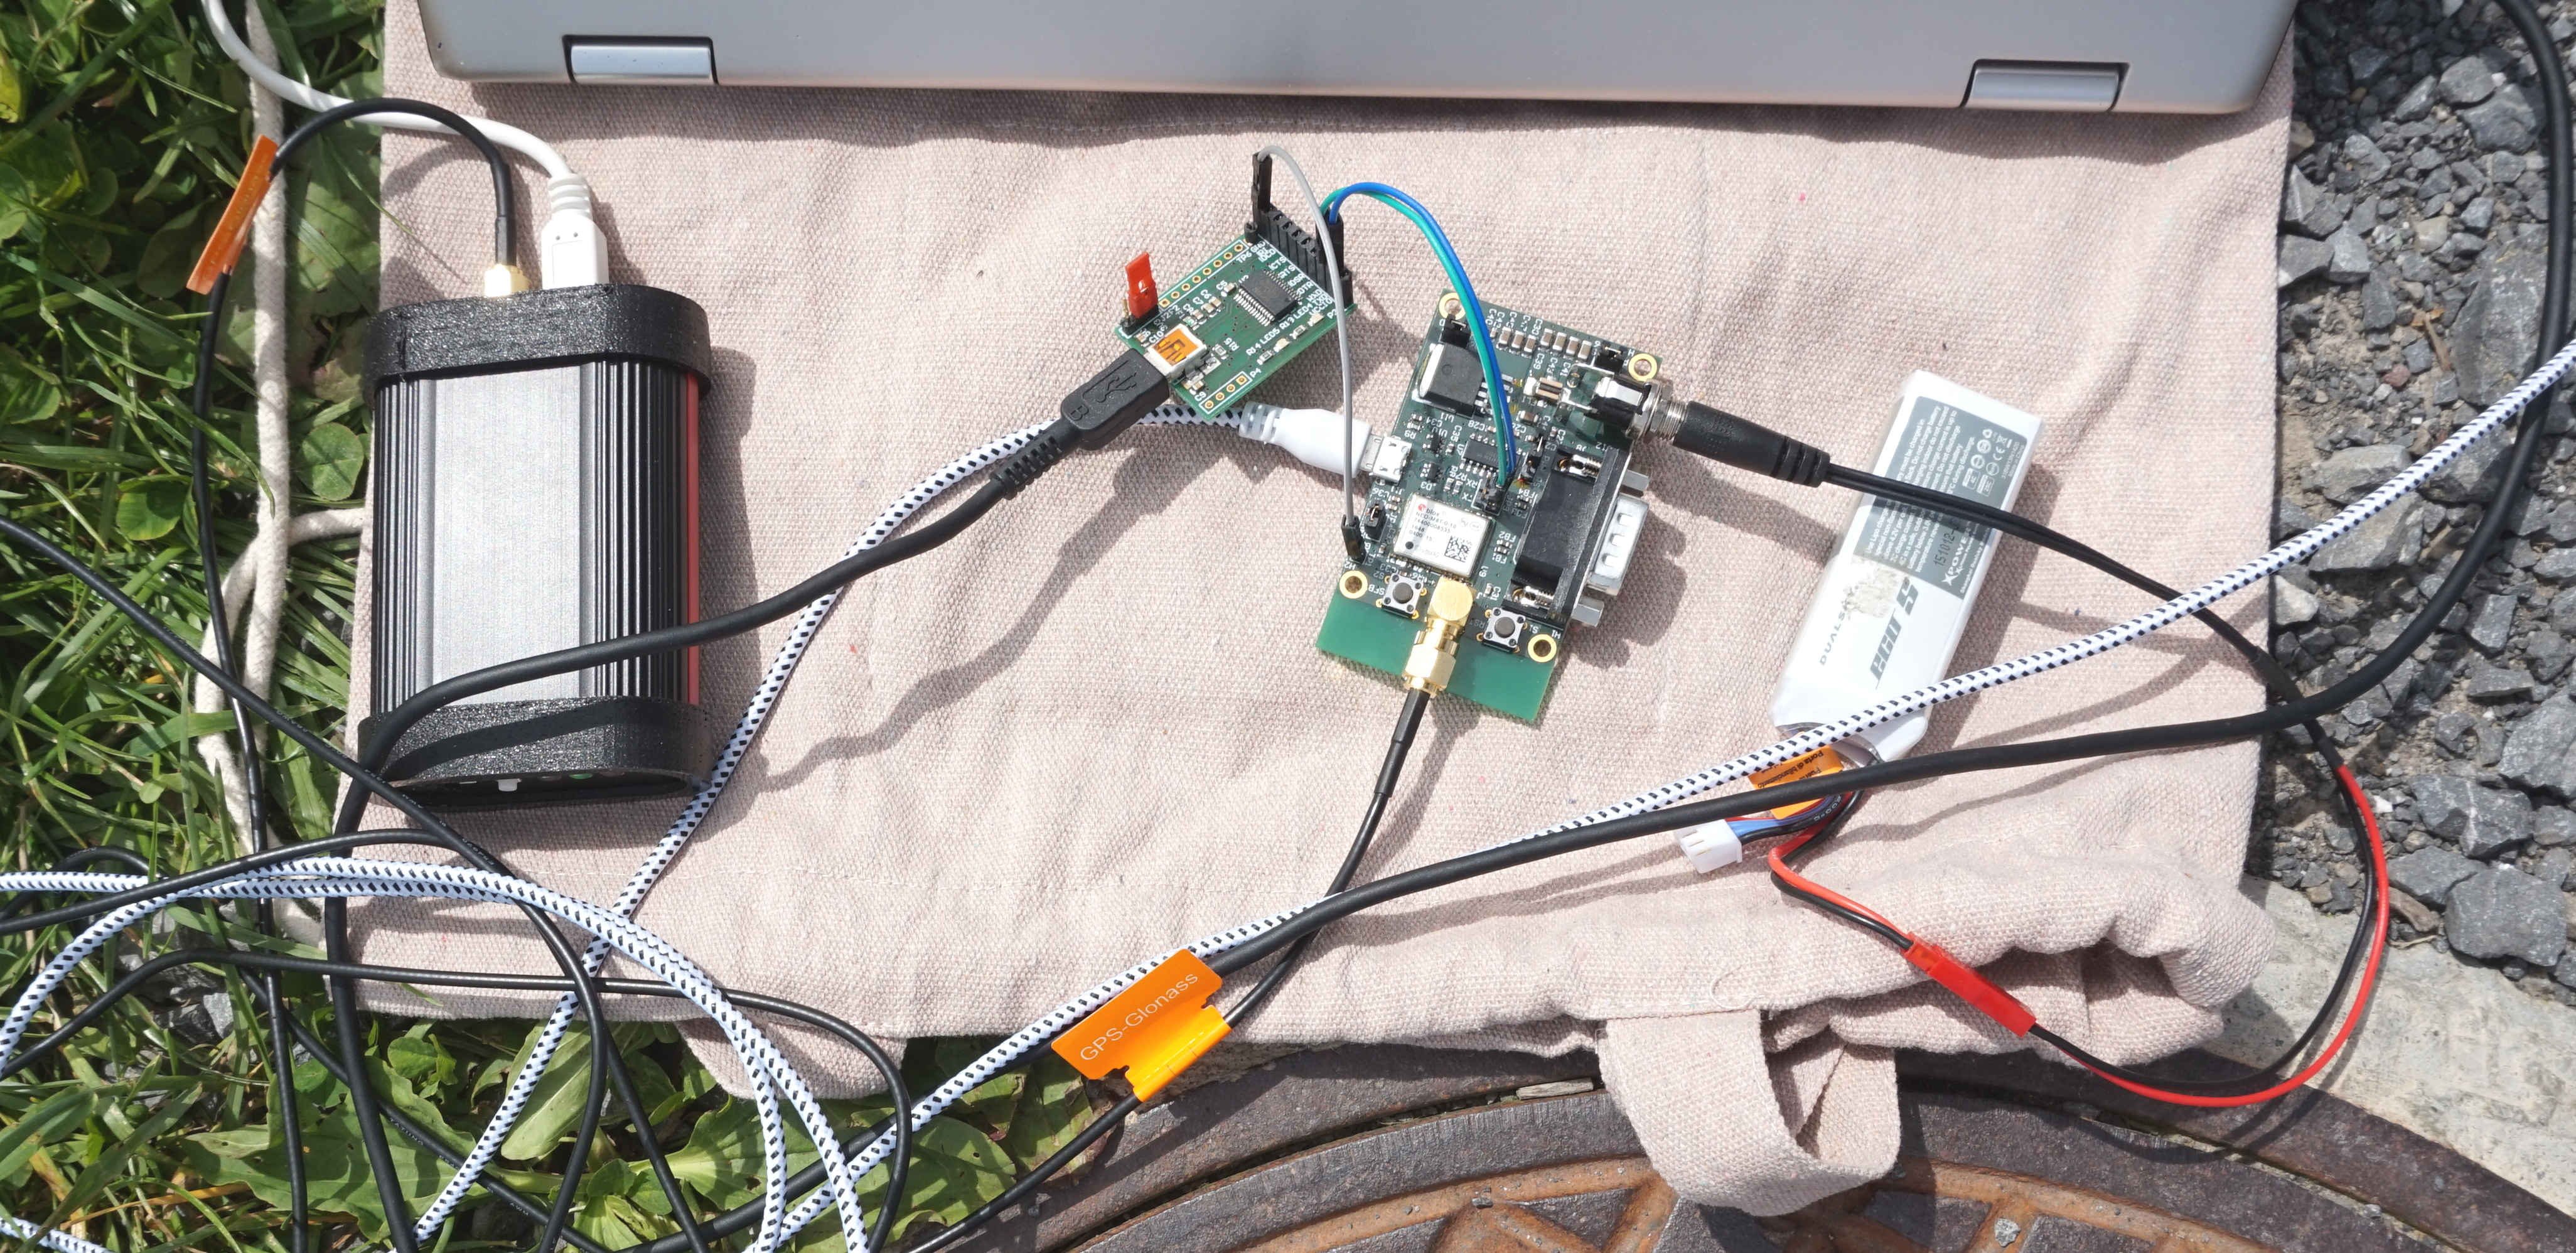
\includegraphics[width=\textwidth]{images/measurement_kriens_receiver.jpg}
 \caption{Receiver setup used for the static accuracy test}
 \label{fig:measurement_kriens_receiver}
\end{figure}

Figure \ref{fig:measurement_kriens_receiver} gives a closer look at the wiring of the receivers.
One M8T receiver is in the black box on the left of the image.
It is used as the reference station and connected to the laptop via USB.
The second M8T receiver, representing the user, is on the GPS board developed by ARIS.
It is powered by a 3 cell LiPo battery and has two serial connections to the laptop.
The first is over USB and used for the RTCM input from the DGPS Message Generator.
The second is an UART connection that is converted to USB with the separate FTDI board.
It is used to have access to the receiver with u-center and monitor its state.

\subsection{Results}

For the evaluation, the measured positions were converted to a local East North Up (ENU) reference frame relative to the reference position.
The scatterplot in figure \ref{fig:scatterplot} shows how the postitions of the two receivers with and without DGPS corrections wandered arround on the horizontal plane.
Standard GPS is in blue and DGPS is in orange.
Imprtant to see is that the middle of the scatterplot is at an offset of about 35 meters in both directions to the reference postition.
  
The large offset in the horizontal plane of both measurements would indicate a wrong reference position.
The calculation of the WGS84 coordinates in ECEF form were double checked with the tool NAVREF from Swisstopo and the Matlab function llh2xyz from appendix \ref{appendix:matlab_code} which gave the same result.

\begin{wrapfigure}{r}{0.5\textwidth}
  \centering
 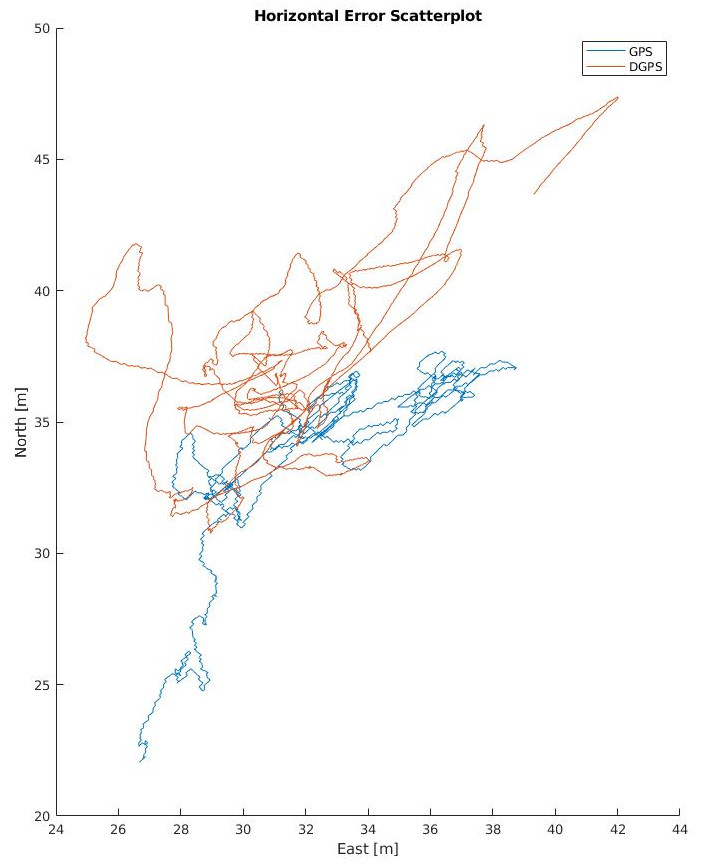
\includegraphics[width=0.5\textwidth]{images/Scatterplot.jpg}
 \captionof{figure}{Scatterplot of the horizontal errors arround the reference position}
 \label{fig:scatterplot}
\end{wrapfigure}

Figure \ref{fig:horizontal_vertical_error} shows the horizontal errors on the left and the vertical errors on the right.
The vertical error of standard GPS is about in the range it could be expected with an RMS error of 11.75 meters.
The horizontal error of standard GPS on the other hand has an RMS error of 45.46 meters.
This is much more than the 10 meter 95th percentile specified in the GPS Performance Stardard.

It is evident that DGPS did not improve those errors distinctly.
Its horizontal error is a bit worse with 49.29 meters RMS and the vertical error a bit better with 8.75 meters RMS than standard GPS.
So there was a small improvement in the vertical error which is the important part of the rocket position for the control.
But it is still far off the 1 meter RMS error defined in the requirements.

Figure \ref{fig:prcs_filtered} shows the PRCs that were calculated by the DGPS Message Generator and applied by the DGPS receiver.
The PRC of 11 GPS satellites were calculated during the test.
About 8 PRCs were available to the DGPS receiver at a time.
They have an average absolute value of 6.8 meters.
The PRC of satellite 2 increaset to -84 meters before is stopped being calculated.
It could be responsible for the increased vertical error of the DGPS solution at arround 1800 seconds.
Such PRCs should be excluded from the RTCM stream in the future.

\begin{figure}[!h]
 \centering
 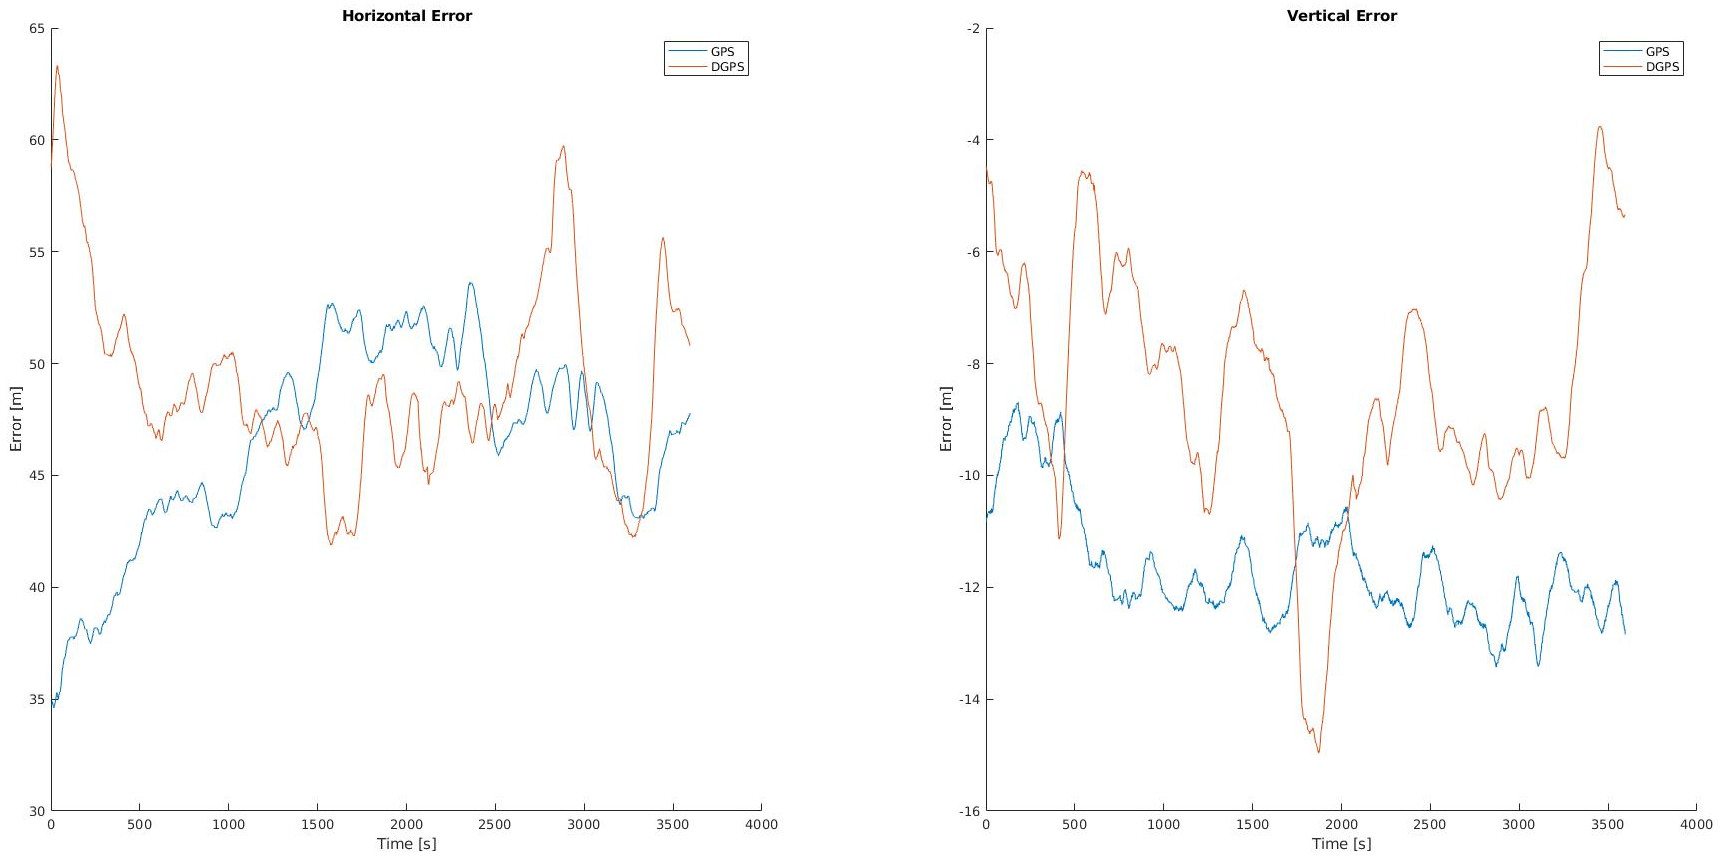
\includegraphics[height=0.4\textheight]{images/Horizontal_Vertical_Error.jpg}
 \caption{Horizontal and vertical errors arround the reference position}
 \label{fig:horizontal_vertical_error}
\end{figure}

\begin{figure}[!h]
 \centering
 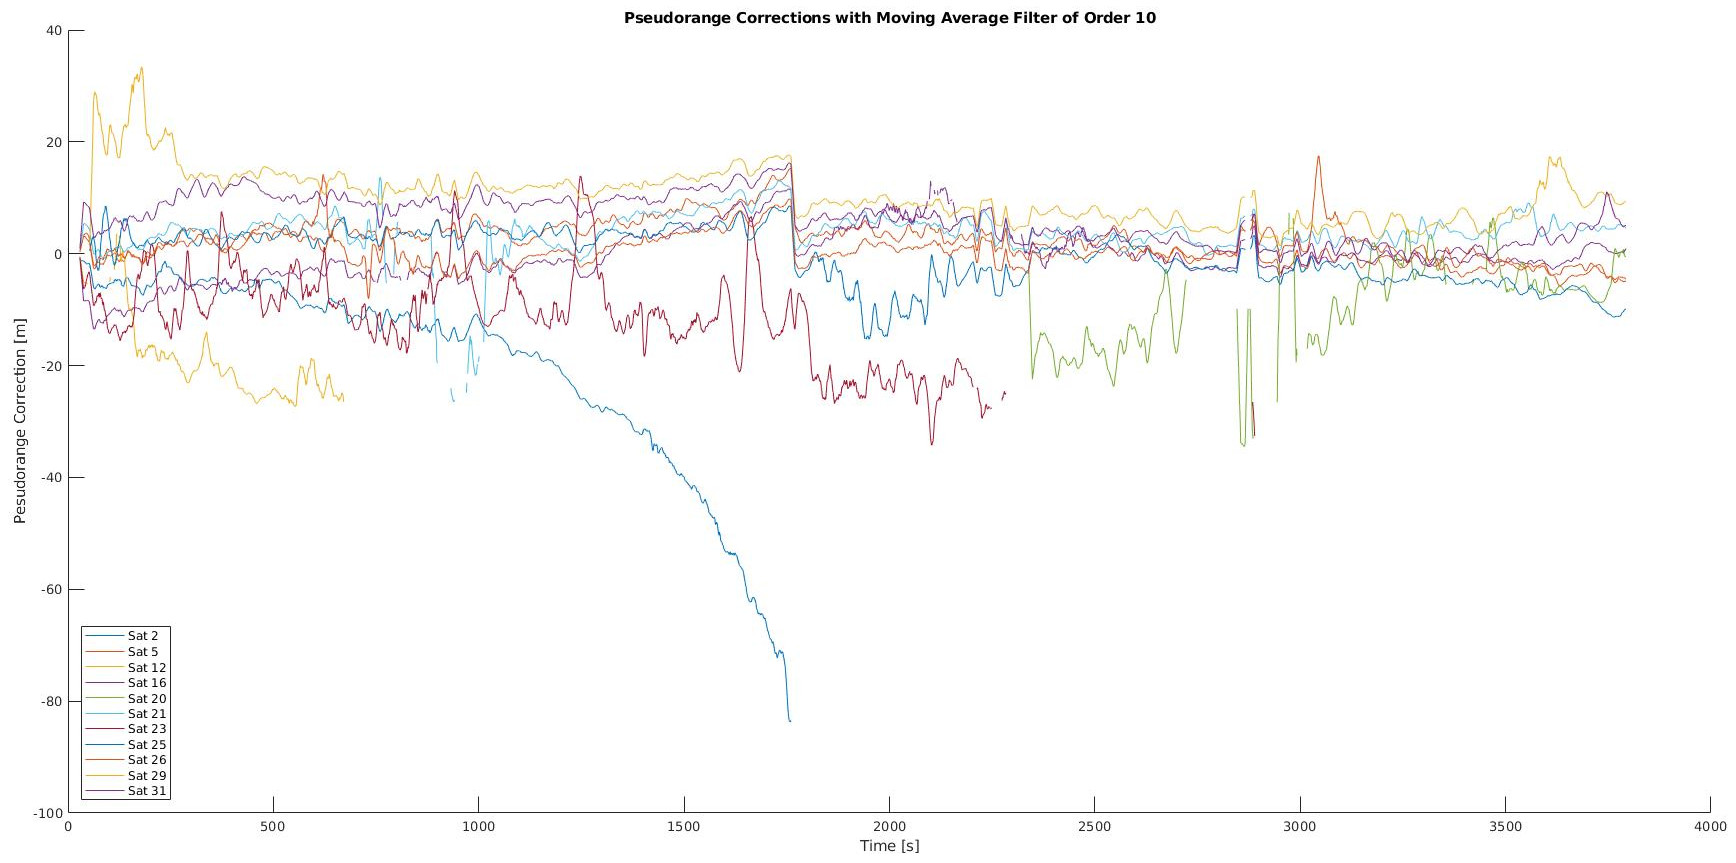
\includegraphics[height=0.4\textheight]{images/PRCs_filtered.jpg}
 \caption{Filtered pseudorange corrections produced by the DGPS Message Generator}
 \label{fig:prcs_filtered}
\end{figure}

\section{Pending Tests}

This secion lists all the tests that were planned but could not be conducted due to time constraints.
Because of the results from the satatic accuracy test, it would also not make sense to test the other scenarios.
The system will probably not produce more accurate results than standard GPS in special conditions when it did not do so in the static test.
The static accuracy would have to be improved first.

\subsection{Mobile Accuracy}

This test is similar to the static accuracy test.
The difference is that the two receivers that estimate the position with and without DGPS corrections move along a pre defined track.
An additional GPS receiver is nedded because the reference receiver can not be used as the standard GPS user anymore.
Also a wireless link is needed to transmit the RTCM stream from the reference station to the user.
The XBee module could be used for this purpose like it was planned for the final implementation.

\subsection{Horizontal Distance}

To measures how well he errors are correlated over a horizontal distance, the reference station and the user will be separated by a distance of about 5 km.
The setup can be the same as in the mobile accuracy test.
The PRCs should still have a positive impact on the position estimation.

\subsection{Height Difference}

A height difference between the reference station and the user can lead to a difference in their tropospheric errors.
If a difference of 3 km has a big impact on the user position accuracy is tested here.
The user receiver is placed on a mountain with a height of about 3 km.
It has a wireless connection to the reference station in the valley.
The range of the XBee module should be sufficient for such a test.
If the height difference has a big impact on the user position accuracy, a differential tropospheric model would have to be added to the PRCs to compensate for it.

\subsection{Telemetry Antenna Interference}

Because the telemetry transmitter on TELL has a transmitting power of 1 W and is placed right next to the GPS antennas, it has to be tested how big its impact on the carrier-to-noise-density ratio is.
With a decrease in the carrier-to-noise-density ratio increases the receiver noise and the position error.
Before it is tested, it should be roughly calculated to make sure the GPS receiver is not damaged.
The test can be done with a standard GPS receiver without DPGS.

\subsection{Antenna Rotation}

Sounding rockets normally rotate to stabilize their trajectory.
A rotation of the GPS antenna can result in a varying signal strenght especially for signals from GPS satellites with low elevations.
It has to be tested how fading affects the GPS receiver.

\subsection{Correction Message Interruption}

During the launch of the rocket, it could come to an interruption of the telemetry link.
This would also interrupt the RTCM stream.
It is tested how long the receiver on the rocket could continue to provide an accurate DGPS position with the old corrections.

\subsection{Rocket Test}

A final validation of the system can only be made with a rocket launch.
Especially if the receiver can handle the acceleration is only possible to test this way.


 
 \chapter{Conclusion}

This final chapter looks back at the project in terms of what has been achieved, how the implemented system can be improved and what still has to be done.


\section{Meeting the objectives}

The assignment for for this project was to evaluate errors that impact the accuracy of GPS positioning and find ways to mitigate them.
The most promising approach should be implementet to show its feasability.
Three groups of errors were found that contain errors in the satellite state, atmospheric modelling and signal reception.
From the three evaluated error correction methods, differential GPS emerged to be the most effective and most suited to implement on a sounding rocket.
A DGPS system was planned to implement on a ARIS sounding rocket and the key component that generates the corrections was developed.
The system was successful at generating correction messages that the user receiver can understand and apply.

Requirements were set in the beginning to specify concrete values by which the success of the project can be deteremined.
The first and most important requirement is about the accuracy of the system.
The vertical RMS error of the position estimation for the rocket should be less than 1 meter.
The current state of the implemented system dose not acieve this.
The static accuracy test showed a vertical RMS error of 8.75 meters.
This is slightly better than the measured standard GPS vertical error of 11.75 meters RMS, but DGPS actually increased the vertical variance from 1.2 to 5 meters.

The second requirement stated that the rocket should have a GPS fix max. 2 seconds after burnout.
DGPS does not pose a problem to achieve this.
It depends on the choosen GPS receiver.
According to the datasheet, the receiver could loose the fix during burn but should be able to get a fix again within 2 seconds.
Only a test can definitively determine if this requirement can be fulfilled.
During this project, no ARIS rocket was launched with GPS onboard.

Finally, a requirement was set to limit the upload bandwith to the rocket that the system can use.
A max. bandwith of 2 kbit/s was defined.
With the RTCM debug output of the DGPS Message Generator, a RTCM message 1 size of 80 bytes was measured to transmit the PRCs of 8 satellites.
A RTCM message 3 is alwasy 30 bytes long.
If both messages are sent twice every second to compensate for the lost messages at the receiver, a bandwidth of only 880 bit/s is used.
It would be sufficient to send RTCM message 3 only once a minute and the frequency of RTCM message 1 could also be reduced if neccessary.


\section{Future Development}

Although the system does not produce satisfying results yet, the underlying functionality of generating corrections and applying them on a receivers position estimation works.
If the integrity of the PRCs could be improved, the system would start to improve the GPS accuracy.
One improvement that could be made to the system is excluding satellites from the PRC calculation if they produce outliners.
It is possible that this behaviour is connected to the elevation of the satellite.
If so, satellites could be excluded based on their elevation.
Another possibility is to estimate the receiver clock offset with a different method.
An often used method is a Kalman Filter.

If the static accuracy is improved, the pending tests from section \ref{sec:pending_tests} can be conducted to validate the functionality of the system in sounding rocket conditions.
To do that, the XBee link has to be implemented first.
The XBee hardware modules have already been built by ARIS.
What is still needed is the interface to the DGPS Message Generator on one side and the interface to the M8T GPS receiver on the other.


\section{Reflection}

It has been an intresting project.
I have learned a lot about GPS of courese, but with that concepts like satellite orbits, reference frames, atmospheric effects on radio waves and CDMA spread spectrum were introduced. 
These are all fascinating topics on their own.

That the proof of concept does not improve the accuracy as expected is a bit dissapointing.
But I think the porject progressed quite far.
With a bit of improvement of the actual PRC calculation algorithm, the system could start to deliver the expected results.

A big thanks on this point to my Supervisor Prof. Marcel Joss and to Dr. Michael Meindl from the Institute of Geodesy and Photogrammetry at the ETH Z\"urich.
I would not have come so far without their help and expertise.

The work on project TELL with the other ARIS team members has been a pleasure.
From the avionics meetings to the test launches and now to see the final rocket.
Although I am not traveling to the U.S. for the competition, I am very excited to see the rocket perform and I wish them all the best.

 
 \bibliography{literatur}
 
 \begin{appendices}
  
  
  
 \end{appendices}
 
\end{document}
